\documentclass[a4paper, 12pt]{article}

\usepackage[utf8]{inputenc}
\usepackage[brazilian]{babel}
\usepackage{graphicx}
\usepackage{amssymb, mathrsfs, amsfonts, amsmath, esint, relsize, bm}
\usepackage{hyperref}
\usepackage{caption}
\usepackage{indentfirst} 
\usepackage{xcolor}
\usepackage{csquotes} % When using babel or polyglossia with biblatex, loading csquotes is recommended to ensure that quoted texts are typeset according to the rules of your main language.
% References
\usepackage[style=ieee]{biblatex}
\addbibresource{refs.bib}

% \usepackage{hhline}
% \usepackage{color}
% \usepackage{soul}
% \usepackage[table,xcdraw]{xcolor}
% \usepackage{enumerate}

%% My commands
% \newcommand{\myref}[1]{{\color{blue} \ref{#1}}} % Display a blue color for linking figures, tables, equations, etc..
% \newcommand{\mywidth}{.6} % Standard for figures
% \hypersetup{linkcolor=blue, filecolor=magenta, urlcolor=cyan}

% Change background color
% \usepackage{pagecolor,lipsum}% http://ctan.org/pkg/{pagecolor,lipsum}

% \definecolor{maroon}{cmyk}{0,0.87,0.68,0.32}

\begin{document}
% \pagecolor{yellow!50!orange} % ``marcador'' de página feita (movimentas ou comentá-lo de acordo com o avanço do trabalho)

%--------------------------------------------------------------------------
% Capa do relatório
\begin{titlepage}
    \begin{center}
        
\includegraphics[width=2cm]{adj/brasao.png}\\
        {\large {Universidade Federal do Ceará}}\\
        {\large {Centro de Tecnologia}}\\
        {\large {Departamento de Engenharia de Teleinformática}}\\
        {\large {Sistemas de Comunicações Digitais - TI0069}}
    \end{center}

    \vspace{100pt}
    
    \begin{center}
        {\large \textbf {Trabalho 01: Modulação Digital}}
    \end{center}
    
    \vspace{100pt}
    
    \begin{table}[h]
    \begin{tabular}{ll}
        \textbf{Aluno:}         &       \\
        Lucas de Souza Abdalah  & 385472
    \end{tabular}
    \end{table}
    
    \begin{table}[h]
    \begin{tabular}{l}
        \textbf{Professor:} André Almeida   \\
        \textbf{Data de Entrega do Relatório:} 28/03/2021
    \end{tabular}
    \end{table}
    
    \vspace{\fill}
    
    \begin{center}
        Fortaleza\\
        2021
    \end{center}
    
    \end{titlepage}
    
    %--------------------------------------------------------------------------
    % Sumario do relatorio
    
    \tableofcontents
    \thispagestyle{empty}
    \clearpage

% ------------------------

\subsection{Problema 1 - \texorpdfstring{$M$}{M}-QAM}

Considere a modulação $M$-QAM, em que o sinal em banda base é dado por:
$$s_m(t) = ( A_m^{(\text{real})} + j A_m^{(\text{imag})}) g(t) ,$$
em que $g(t)$ é um pulso transmitido, $A_m^{(\text{real})}$ e $A_m^{(\text{imag})}$ são amplitudes da parte real e imaginária da forma de onda transmitida, respectivamente.

% Considere $\int_{-\inf}^{\inf} |g(t)|^2 \,dt = \mathcal{E}_{g} = 1$, isto é, o pulto $g(t)$ possui energia unitária. Suponha a transmissão de uma sequência de símbolo $\{s_{m}\}$ de tamanho $L = 26400 \text{bits}$
% \begin{enumerate}
%     \item A energia média $\mathcal{E}_{m}$ de cada constelação;
%     \item A distância mínima $d_{min}$ entre dois símbolos;
%     \item O modulador (mapeamento bit-símbolo) usando a codificação de Gray;
%     \item O demodulador (mapeamento símbolo-bit).
% \end{enumerate}

% -------------------------------------------------------------------

\subsubsection{Energia da Constelação} 

O desenvolvimento é citado em~\cite{Proakis, Cecilio}.

$$ \mathcal{E}_{media} = \frac{M-1}{3} \mathcal{E}_g$$

$$ \mathcal{E}_{media(bit)} = \frac{M-1}{3\log_2 M} \mathcal{E}_g $$
% -------------------------------------------------------------------
\subsubsection{Distância Mínima entre Símbolos}

Como calcular os coeficiente para constelação $M$-QAM retangular, onde $\sqrt{M}$ assume valores inteiros. Os coeficientes em quadratura $a_i$ e $b_i$ são obtidos através da equação: $\{ (2i -\sqrt{M} - 1)d \}_{i=1}^{\sqrt{M}} $ 

A distância eucliadiana entre os sinais na modulação QAM é
$$ d_{mn} = \sqrt{|| s_m - s_n||^2}$$ 
$$ = \sqrt{\frac{\mathcal{E}_g}{2}[(A_{mi} - A_{ni})^2 + (A_{mq} - A_{nq})^2]}$$

$$\sqrt{\frac{3 \mathcal{E}_{media}}{2(M-1)}} $$

\begin{table}[!ht]
    \centering
    \begin{tabular}{|c|c|c|c|}
    \hline
    $M$-QAM & $\mathcal{E}_{media}$ & $\mathcal{E}_{media(bit)}$ & $d$ \\ \hline
    & &  &  \\ 
    $M$ & $\frac{M-1}{3} \mathcal{E}_g$ & $ \frac{M-1}{3\log_2 M} \mathcal{E}_g$ & $\sqrt{\frac{3 \mathcal{E}_{media}}{2(M-1)}} $ \\ 
    & &  &  \\ \hline
    & &  &  \\ 
    $4$     & 1 & $1.67\times 10^{-1}$ & $\frac{\sqrt{2}}{2}$ \\ 
    & &  &  \\ \hline
    & &  &  \\ 
    $16$    & 5 & $4.67\times 10^{-1}$ & $\frac{\sqrt{2}}{2}$ \\ 
    & &  &  \\ \hline
    & &  &  \\ 
    $64$    & 21 & $1.17\times 10^{0}$ & $\frac{\sqrt{2}}{2}$ \\
    & &  &  \\ \hline
    \end{tabular}
    \caption{Informações gerais calculadas para a modulação $M$-QAM.}
    \label{tab:Resume_QAM}
\end{table}

\clearpage

\subsubsection{Modulador (Codificação de Gray)}

\begin{figure}[!ht]
    \centering
    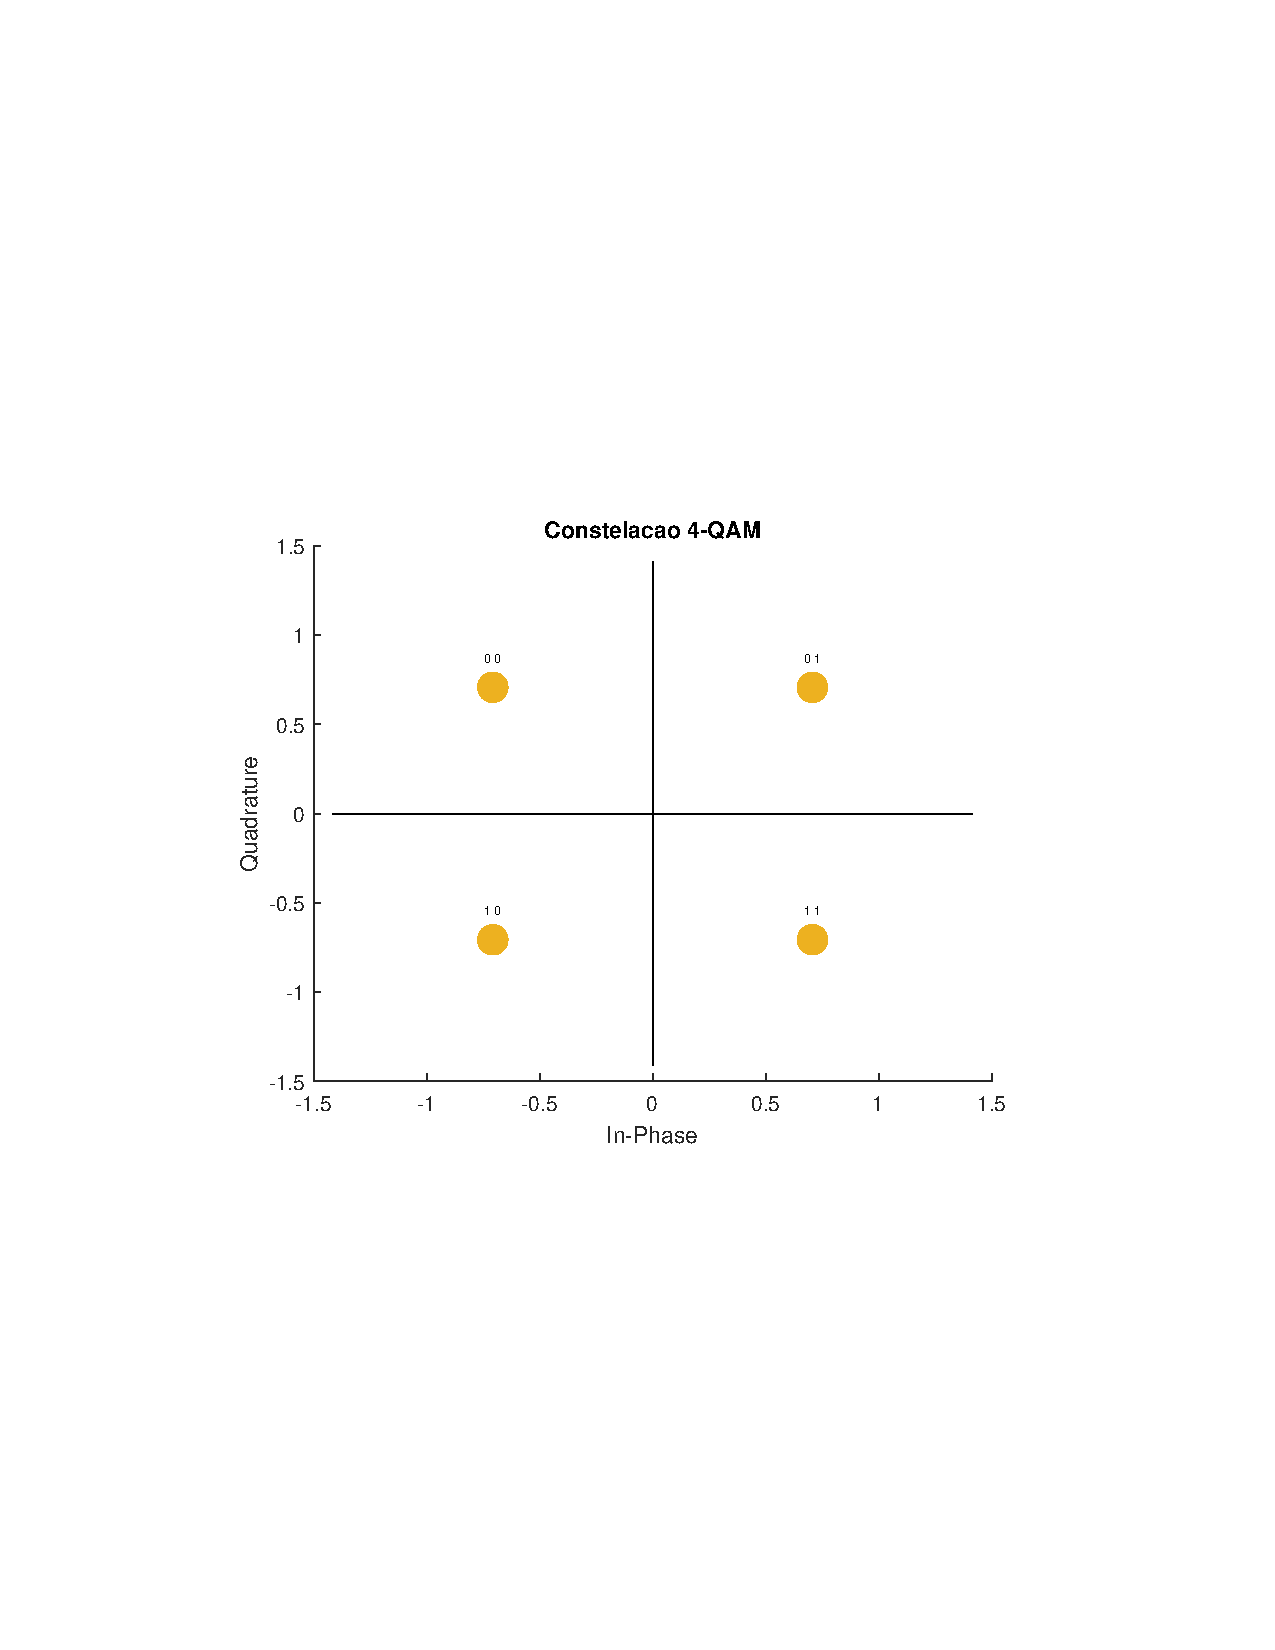
\includegraphics[width=1.0\textwidth,clip=true,trim={1.5cm 8.5cm 1.8cm 8.3cm}]{C:/Users/lukin/Documents/GitHub/Courses-HWs/Sistemas de Comunicacoes Digitais/matlab/problema1/fig/4_QAM_plot.pdf}
    \caption{Exemplo de 4-QAM plot.}
    \label{fig:4_QAM_plot}
\end{figure}

\begin{table}[!ht]
    \centering
    \begin{tabular}{|c|c|c|c|}
    \hline
    Decimal & Binário & Gray & Decimal \\ \hline
    0 & 00 & 00 & 0\\ \hline
    1 & 01 & 01 & 1\\ \hline
    2 & 10 & 11 & 3\\ \hline
    3 & 11 & 10 & 2\\ \hline
    \end{tabular}
    \caption{Tabela de tradução de binário para Gray com 2 bits.}
    \label{tab:Alfabeto_Gray}
\end{table}

Algoritmo para obter o código de Gray~\ref{alg:Gray}

% global change
\SetKwInput{KwData}{Entrada}
\SetKwInput{KwResult}{Saída}

\begin{algorithm}[!ht]
    \SetAlgoLined
    \KwData{Sequência de Bits $(b)$ - MSB}
    \KwResult{Sequencia em Código Gray $(g)$ - LSB}
    $n = 0$\;
    $K = \text{length}(b)$\;
    \While{$K > n$}{
        \eIf{$K==n$}{
            $g_{(K-n)} = b_{(K-n)}$ \;
            }{
            $g_{(K-n)} = b_{(K-n+1)} \otimes b_{(K-n)}$\;
        }
        $n=n+1$;\;
     }
     $g = flip(g)$\;
     \caption{Codificação de Gray}
     \label{alg:Gray}
\end{algorithm}

\clearpage



\begin{figure}[!ht]
    \centering
    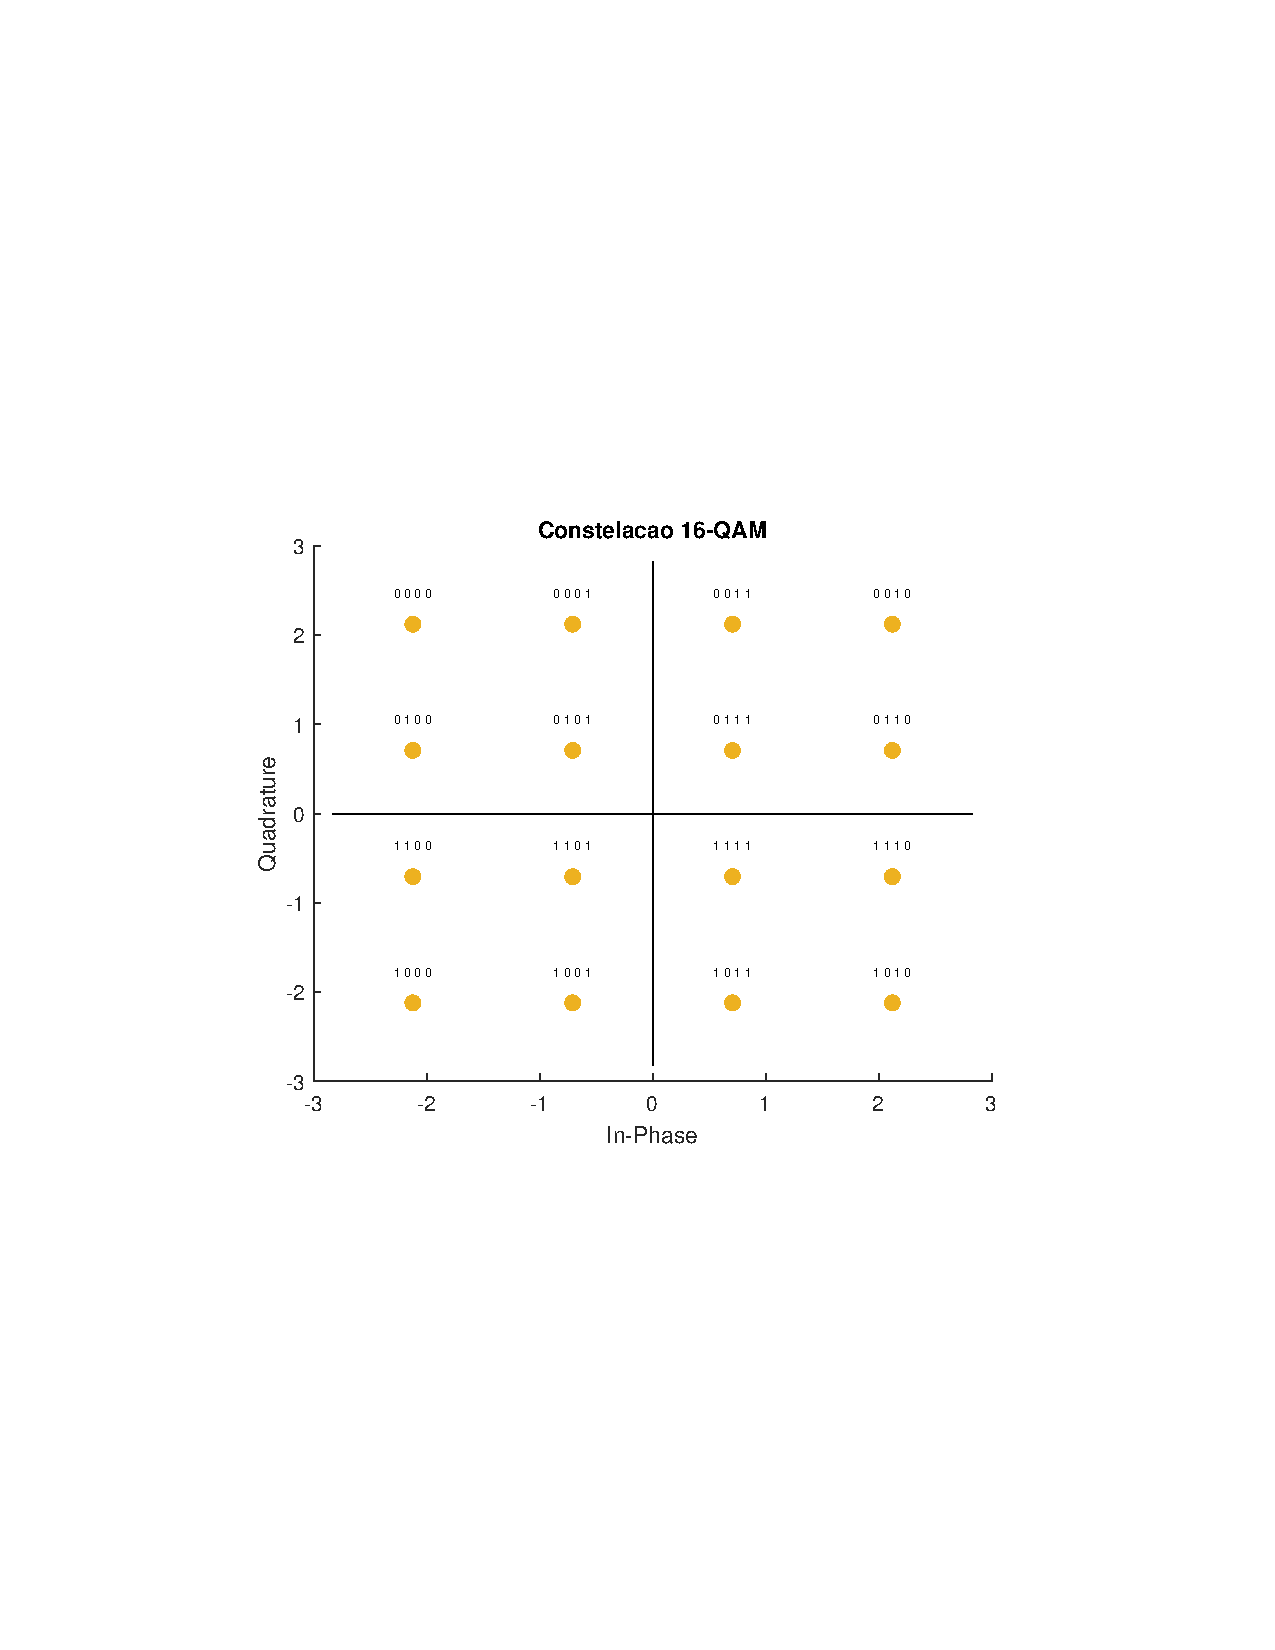
\includegraphics[width=1.0\textwidth,clip=true,trim={1.5cm 8.5cm 1.8cm 8.3cm}]{C:/Users/lukin/Documents/GitHub/Courses-HWs/Sistemas de Comunicacoes Digitais/matlab/problema1/fig/16_QAM_plot.pdf}
    \caption{Exemplo de 16-QAM plot.}
    \label{fig:16_QAM_plot}
\end{figure}

\begin{figure}[!ht]
    \centering
    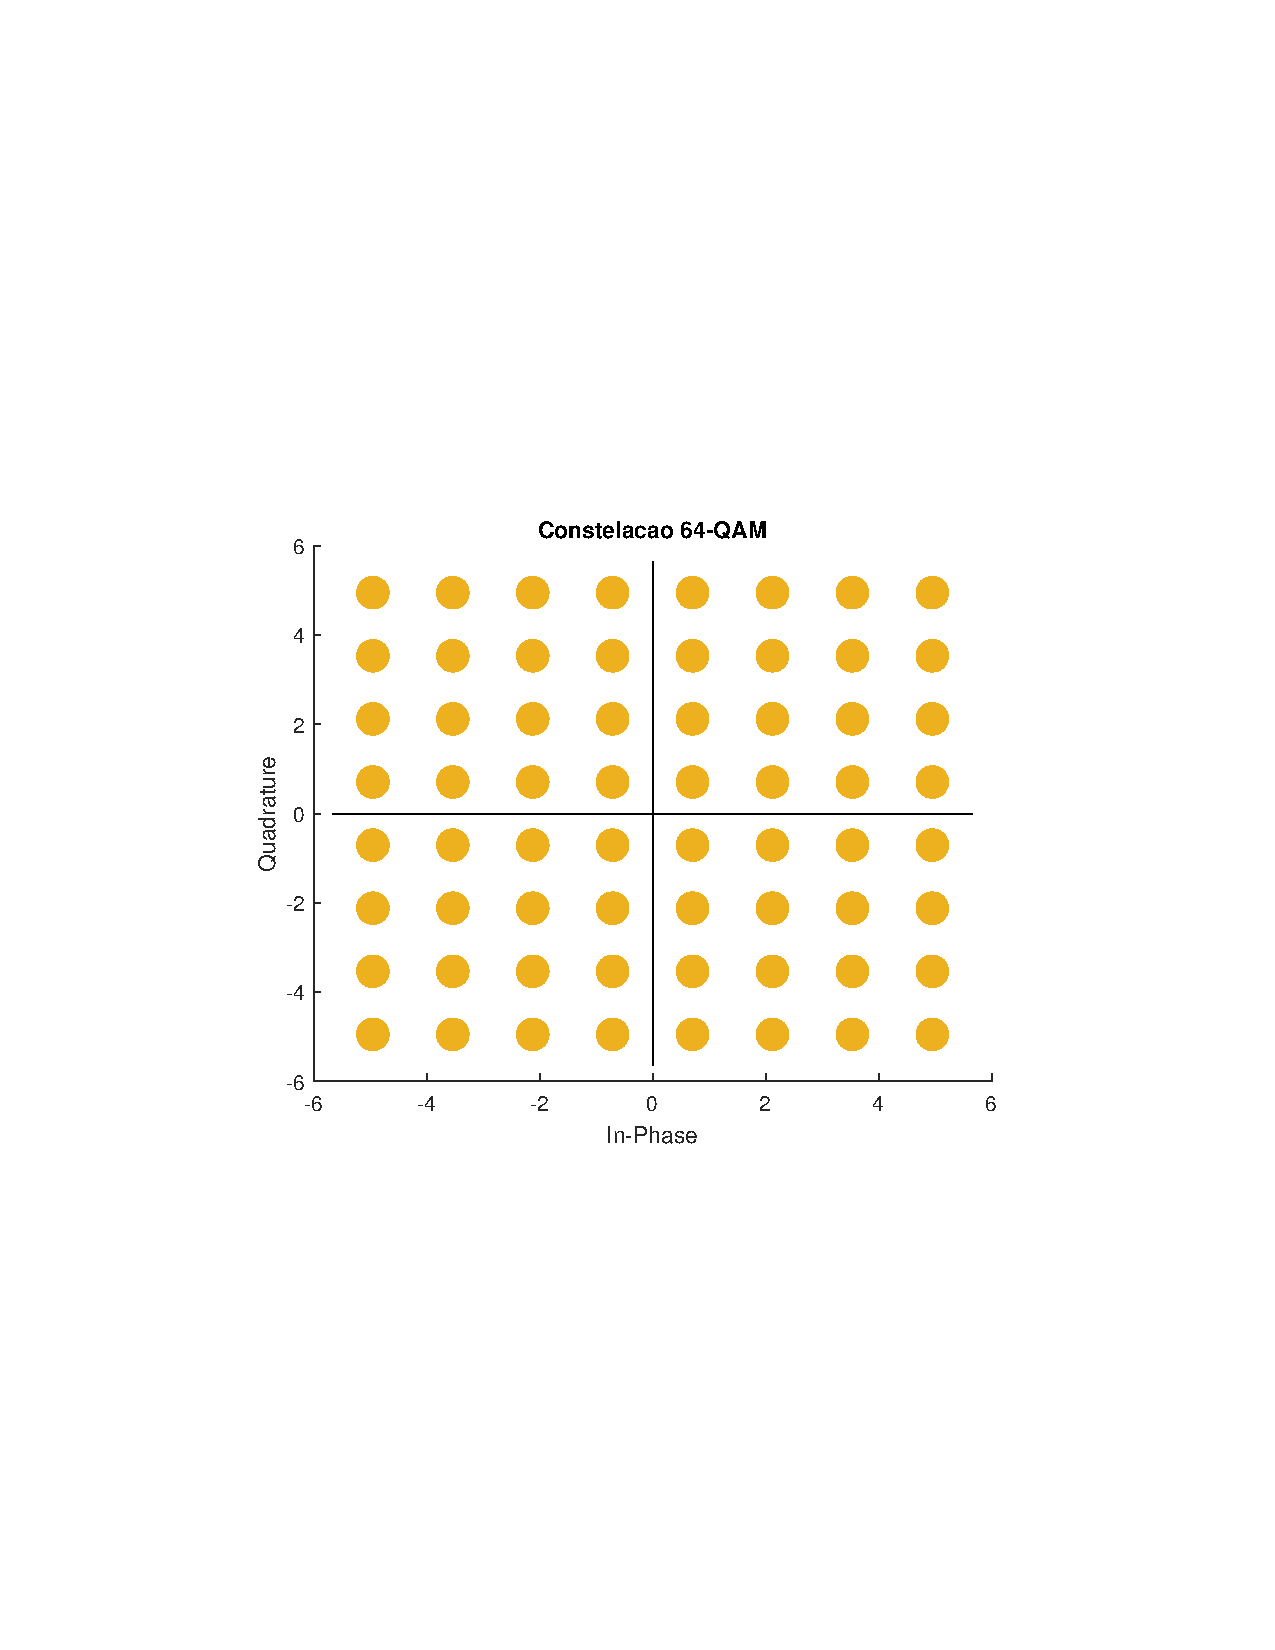
\includegraphics[width=1.0\textwidth,clip=true,trim={1.5cm 8.5cm 1.8cm 8.3cm}]{C:/Users/lukin/Documents/GitHub/Courses-HWs/Sistemas de Comunicacoes Digitais/matlab/problema1/fig/64_QAM_plot.pdf}
    \caption{Exemplo de 64-QAM plot.}
    \label{fig:64_QAM_plot}
\end{figure}

\clearpage

% -------------------------------------------------------------------
\subsubsection{Demodulador}

Considerando $\mathcal{E}_g = \int_{-\infty}^{\infty} |g(t)|^2 \,dt = 1$, a energia média da constelação pode ser calculada por $\epsilon$



%%
% Please add the following required packages to your document preamble:

\clearpage

Para calcular a probabilidade de erro $P(e)$ de cada constelação~\ref{eq:Pe_M_QAM} desenvolvida em~\cite{Cecilio}.
\begin{equation}
    P(e) = 4 \left(1-\frac{1}{\sqrt{M}}\right) Q\left(\sqrt{\frac{3}{M-1}\frac{E_s}{N_0}}\right) - 4\left(1-\frac{1}{\sqrt{M}}\right)^2 Q^2\left(\sqrt{\frac{3}{M-1}\frac{E_s}{N_0}}\right)
    \label{eq:Pe_M_QAM}
\end{equation}

Para valores mais elevados de \textit{SNR}, a equação da probabilidade do $M$-QAM pode ser reduzida para~\ref{eq:Pe_reduzida_M_QAM}, pois o segundo termo ao quadrado passa a ser irrelevante.
\begin{equation}
    P(e) = 4 \left(1-\frac{1}{\sqrt{M}}\right) Q\left(\sqrt{\frac{3}{M-1}\frac{E_s}{N_0}}\right)
    \label{eq:Pe_reduzida_M_QAM}
\end{equation}

\clearpage
\section{Problema 3 - Canal RAGB: \texorpdfstring{$M$}{M}-QAM}
\subsection{Modelo}
Considerando que um sinal ($s_m$) de mensagem passa por um canal de Ruído Adivitivo Gaussiano Branco (RAGB), o modelo da Equação~\ref{eq:AWGM_Model}, onde como uma variável aleatoria, $\mathcal{C} \mathcal{N} (0,N_0)$, Gaussiana complexa com média zero e variância $N_0$. 
\begin{equation}
    y_m = s_m + n_m
    \label{eq:AWGM_Model}
\end{equation}

A variância é dada por $\sigma_{n}^{2} = \frac{N_0}{2}$, representando a potência média do ruído que afeta cada dimensão do sinal em banda base~\cite{Proakis}. Consequentemente, o desvio padrão do ruído corresponde a $\sqrt{\frac{N_0}{2}}$, poderando parte real e imaginária. Portanto, tendo um valor de SNR ($E_s\_N_0$) em dB, o termo $N_0$ pode ser calculado por $N_0= E_s 10^{-\frac{E_s\_N_0}{10}}$, tendo enfim o termo $n_m$ é obtido na equação~\ref{eq:termo_ruido}.
\begin{equation}
    n_m = \sqrt{\frac{N_0}{2}} \left(\text{randn}(1) + 1j \text{randn}(1)\right)
    \label{eq:termo_ruido}
\end{equation}

Para ilustrar a implementação do modelo, as constelações $M$-QAM recebem uma sequência de símbolos com SNR de 25dB gerados no script \href{https://raw.githubusercontent.com/lucasabdalah/Courses-HWs/SCD/Sistemas%20de%20Comunicacoes%20Digitais/matlab/problema3/script_AWGN.m}{\colorbox{cyan!10}{script\_AWGN.m}}, como mostrado na figura~\ref{fig:4QAM_25dB}, \ref{fig:16QAM_25dB} e \ref{fig:64QAM_25dB}.

\begin{figure}[!ht]
    \centering
    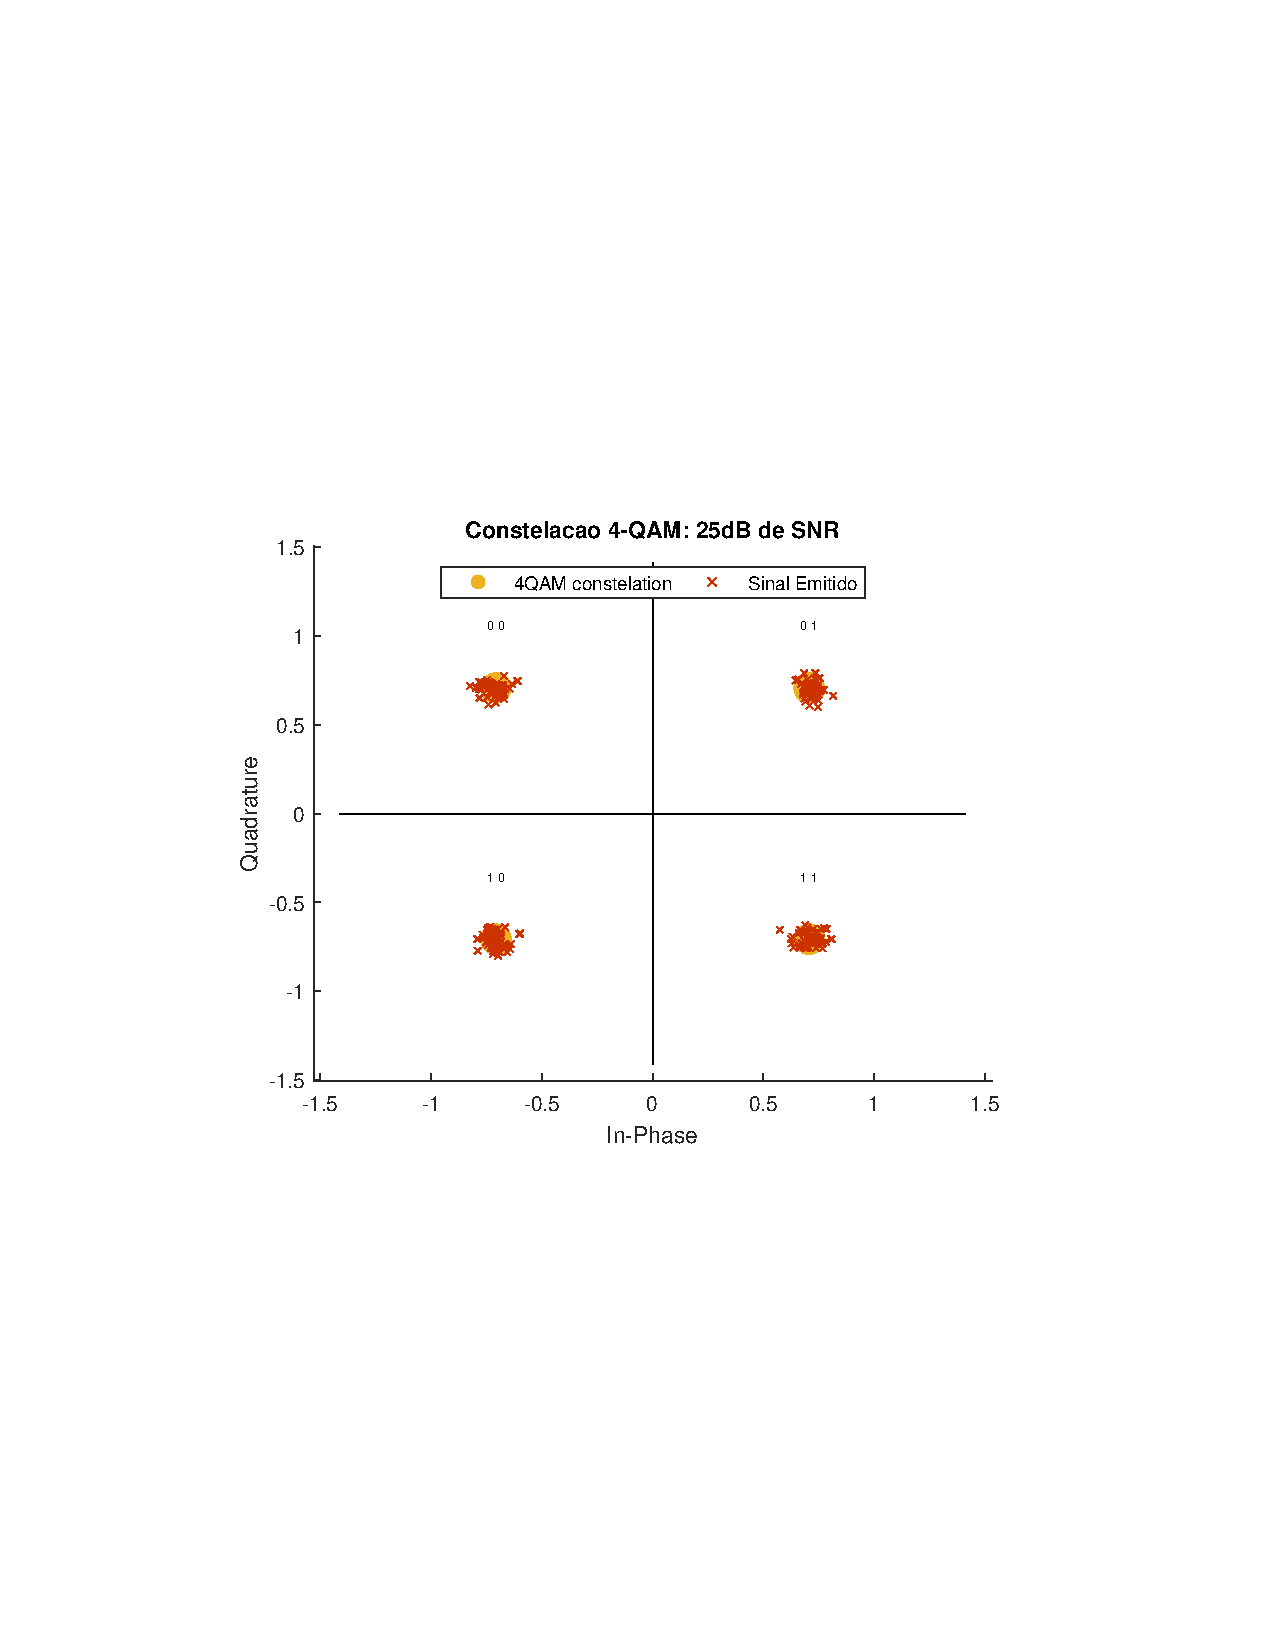
\includegraphics[width=1.0\textwidth,clip=true,trim={1.5cm 8.5cm 1.8cm 8.3cm}]{C:/Users/lukin/Documents/GitHub/Courses-HWs/Sistemas de Comunicacoes Digitais/matlab/problema3/fig/4QAM_25dB.pdf}
    \caption{Simulação de transmissão $4$-QAM, com \textit{SNR} de 25dB.}
    \label{fig:4QAM_25dB}
\end{figure}

\begin{figure}[!ht]
    \centering
    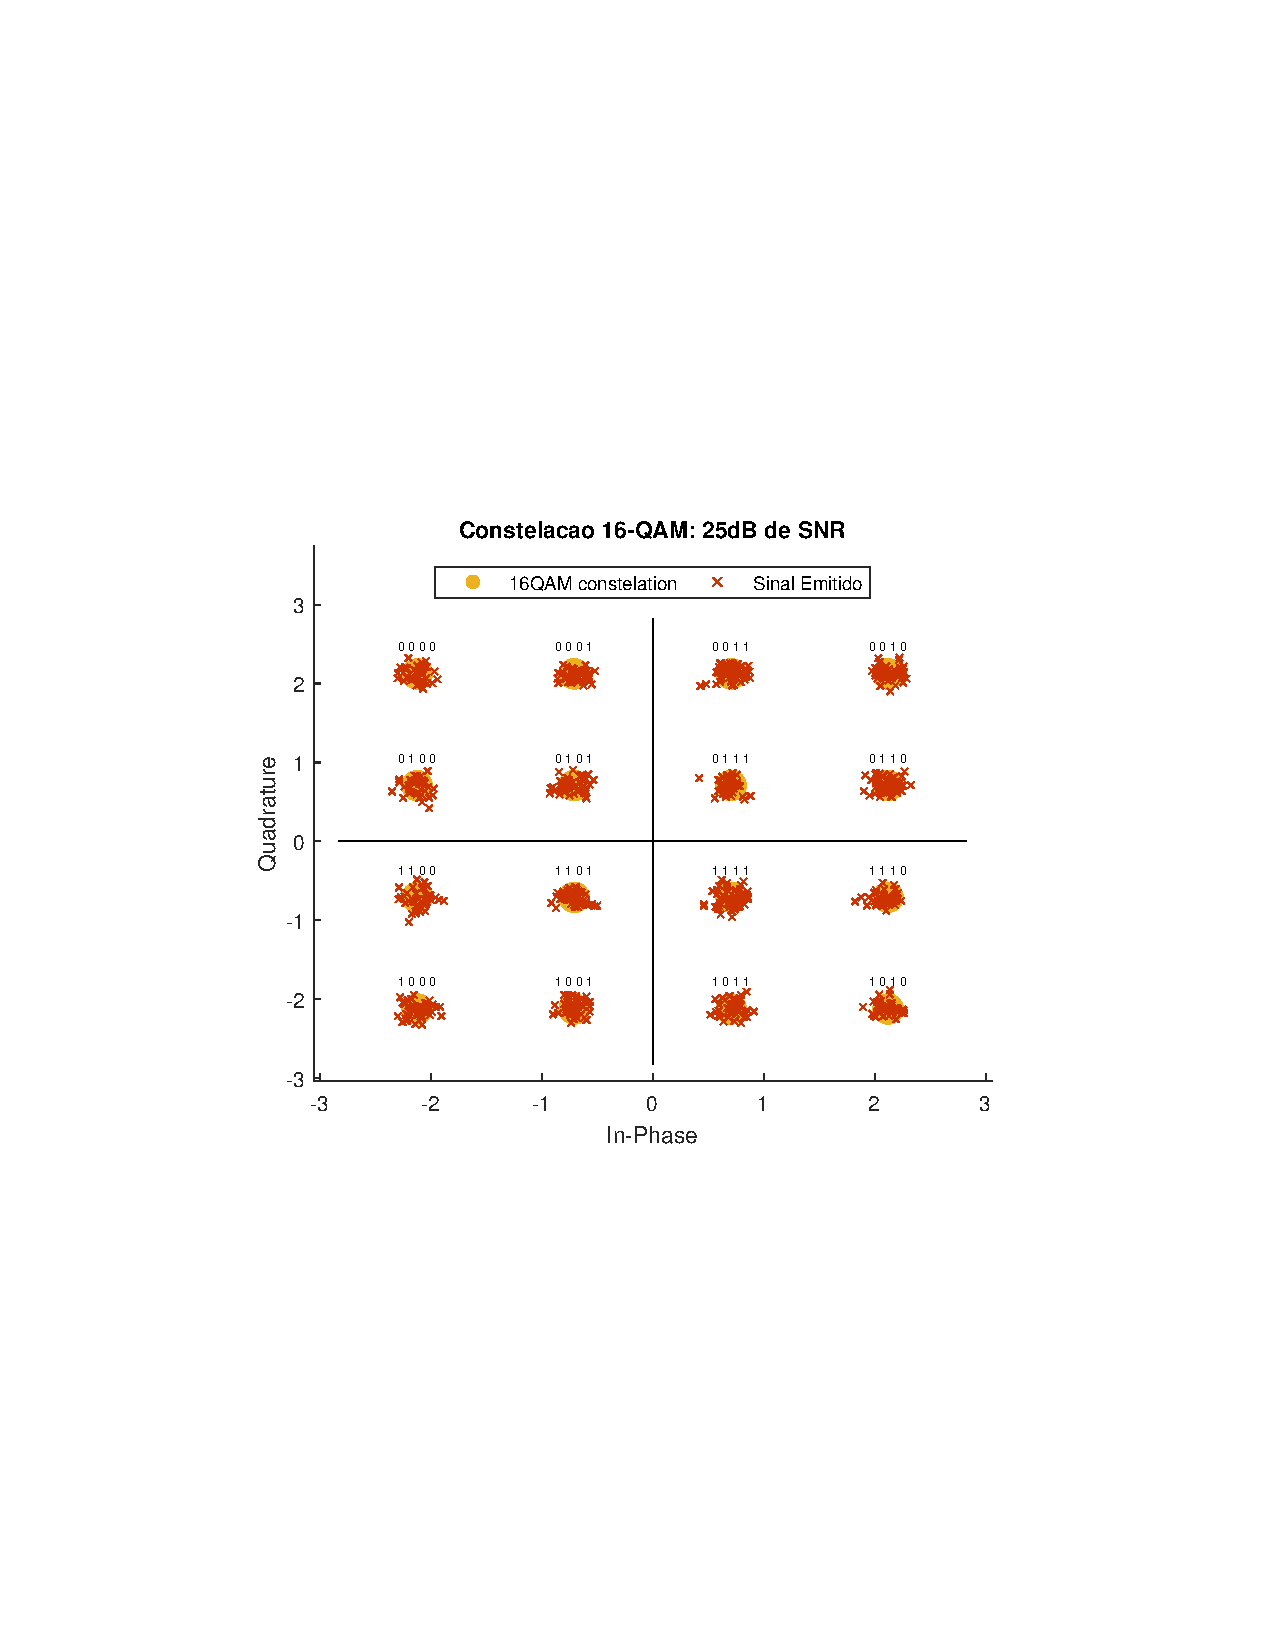
\includegraphics[width=1.0\textwidth,clip=true,trim={1.5cm 8.5cm 1.8cm 8.3cm}]{C:/Users/lukin/Documents/GitHub/Courses-HWs/Sistemas de Comunicacoes Digitais/matlab/problema3/fig/16QAM_25dB.pdf}
    \caption{Simulação de transmissão $16$-QAM, com \textit{SNR} de 25dB.}
    \label{fig:16QAM_25dB}
\end{figure}

\begin{figure}[!ht]
    \centering
    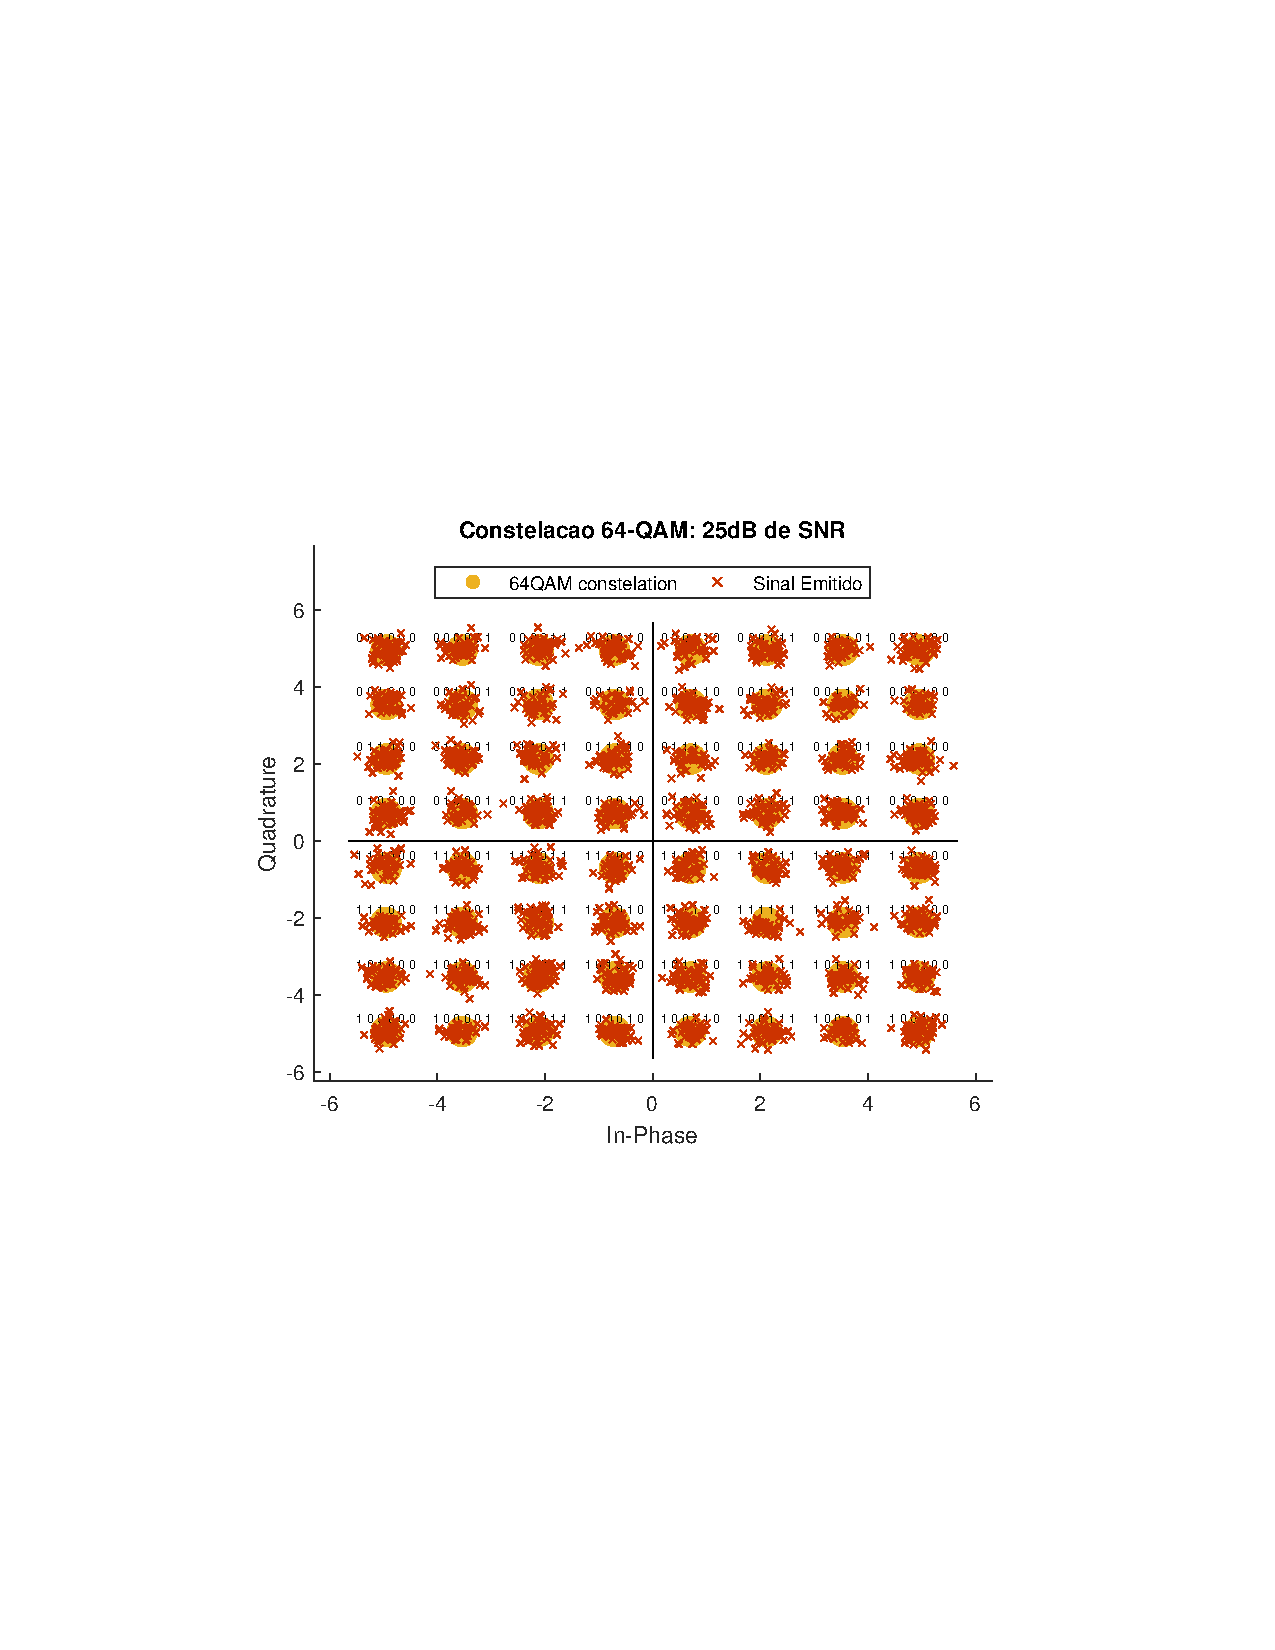
\includegraphics[width=1.0\textwidth,clip=true,trim={1.5cm 8.5cm 1.8cm 8.3cm}]{C:/Users/lukin/Documents/GitHub/Courses-HWs/Sistemas de Comunicacoes Digitais/matlab/problema3/fig/64QAM_25dB.pdf}
    \caption{Simulação de transmissão $64$-QAM, com \textit{SNR} de 25dB.}
    \label{fig:64QAM_25dB}
\end{figure}

\clearpage

\subsection{Experimento de Transmissão}

 O experimento consiste em realizar uma transmissão de uma sequência $s_m$ de tamanho $L = 264000 \text{bits}$ pelo modelo do canal RAGB com as constelações $M$-QAM, variando a \textit{SNR} de 0 a 20 dB com passo 2.

Ao traçar as curvas teóricas de probabilidade de erro de símbolo $P(e)$ e a taxa de erro de símbolo \textit{SER} na figura~\ref{fig:Erro_teoricaxAWGN_MQAM} é possível observar que os valores teóricos e simulados são idênticos, corroborando o embasamento desenvolvido nas seções anteriores.

Estes resultados são gerados com a rotina \href{https://raw.githubusercontent.com/lucasabdalah/Courses-HWs/SCD/Sistemas%20de%20Comunicacoes%20Digitais/matlab/problema3/script_teoricaxAWGN.m}{\colorbox{cyan!10}{script\_teoricaxAWGN.m}}, que chama os dados já computados nas seções anteriores e traça as curvas em um mesmo gráfico.

\begin{figure}[!ht]
    \centering
    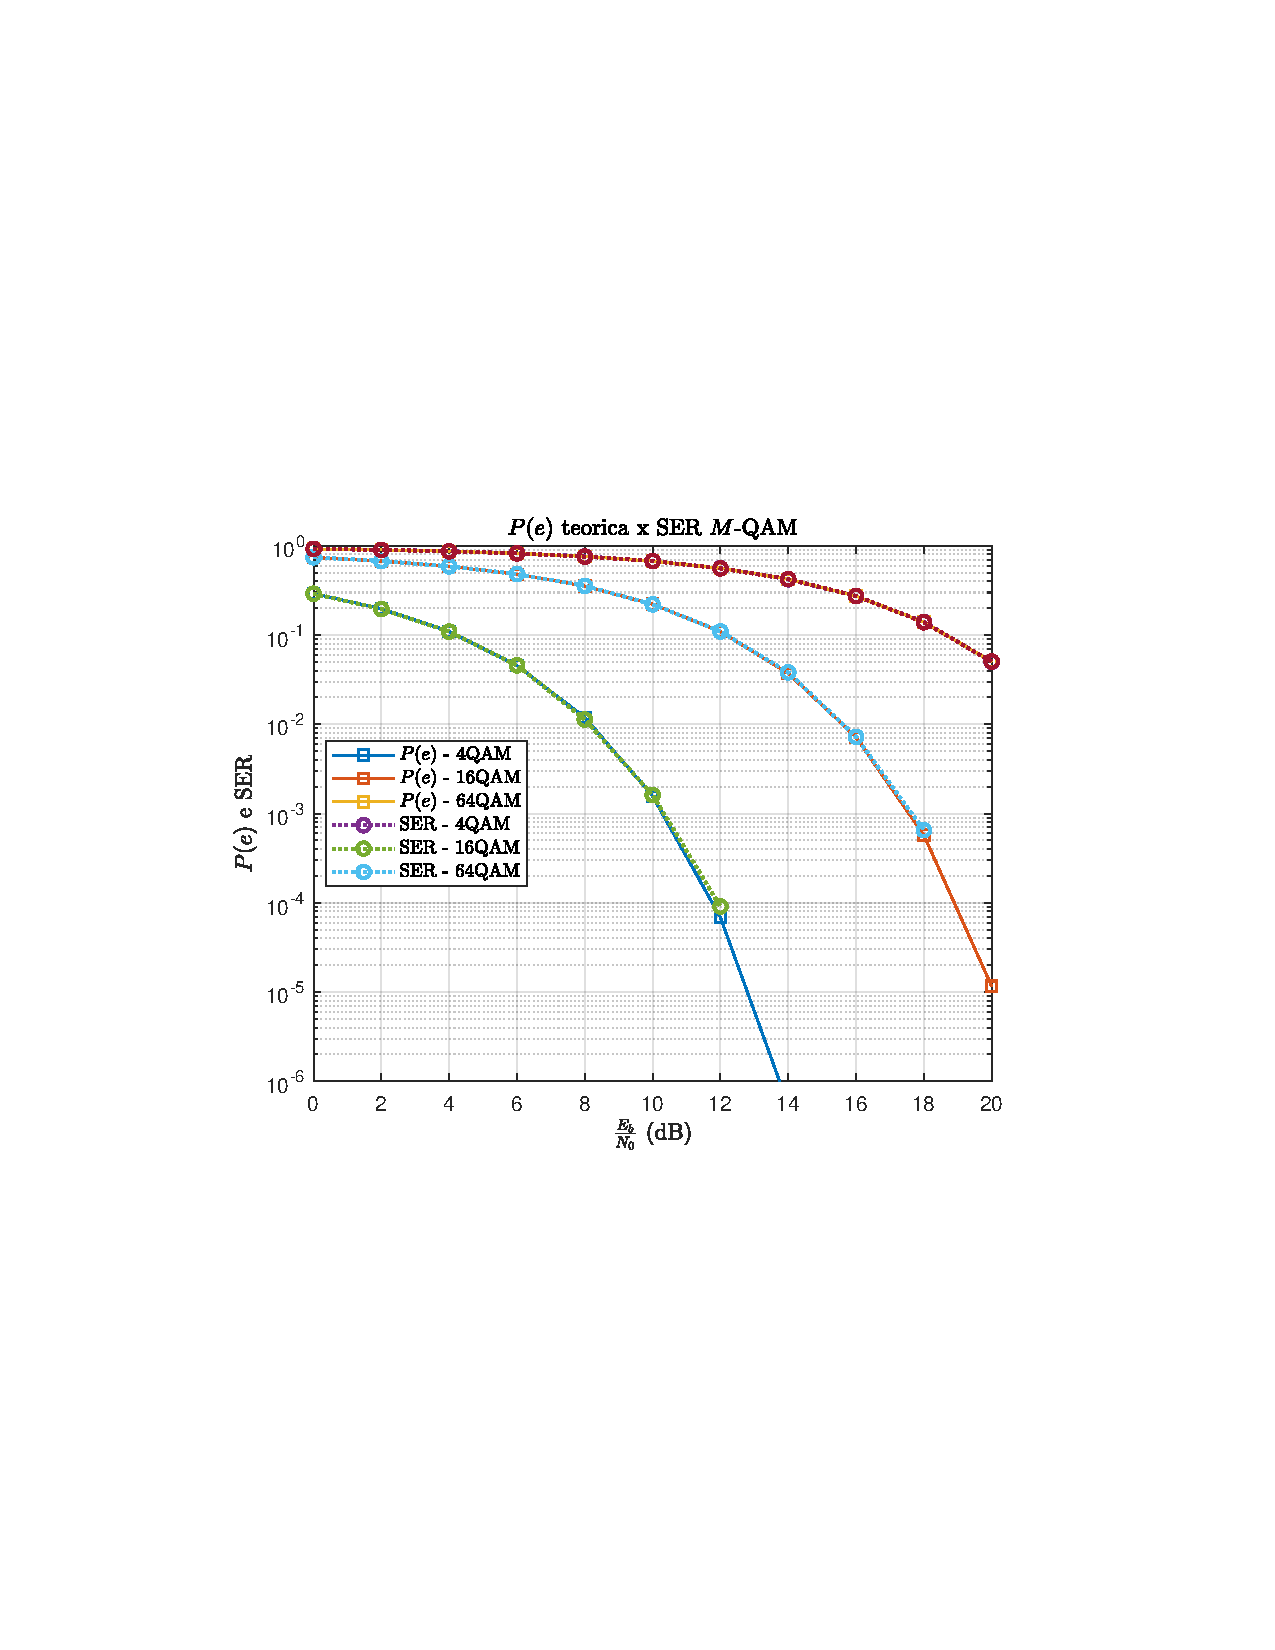
\includegraphics[width=1.0\textwidth,clip=true,trim={1.5cm 8.5cm 1.8cm 8.3cm}]{C:/Users/lukin/Documents/GitHub/Courses-HWs/Sistemas de Comunicacoes Digitais/matlab/problema3/fig/Erro_teoricaxAWGN_MQAM.pdf}
    \caption{Probabilidade teórica de erro vs. simulação de transmissão $M$-QAM em canal RAGB.}
    \label{fig:Erro_teoricaxAWGN_MQAM}
\end{figure}
\clearpage
\section{Problema 4 - Modulação \texorpdfstring{$M$}{M}-PSK}

O conjunto de sinais \textit{phase-shift keying} (PSK) têm a mesma amplitude e fases diferentes para cada mensagem, podendo ser escrito para $M > 2$ de acordo com a equação~\ref{eq:PSK_si}
\begin{equation}
    s_i(t) = \sqrt{\frac{2\mathcal{E}_s}{\mathcal{E}_g}} g(t) cos(2\pi f_c t + \frac{(2i-1)\pi}{M}), \, 0 \leq t \leq T, \, i = 1,2,\dots,M,
    \label{eq:PSK_si}
\end{equation}

Assumindo a energia do pulso de transmissão unitária, $g(t) = 1$, o sinal também pode ser expresso através de uma combinação linear~\cite{Cecilio}, de modo que $s_i(t)$ é reescrito coom na equação~\ref{eq:PSK_simbolos}
\begin{equation}
    s_i =   \begin{bmatrix}
                \sqrt{\mathcal{E}_s} cos(\frac{(2i-1)\pi}{M}) \\
                \\ 
                \sqrt{\mathcal{E}_s} sin(\frac{(2i-1)\pi}{M}) \\ 
            \end{bmatrix}, \, i = 1,\dots,M
    \label{eq:PSK_simbolos}
\end{equation}

A função \href{https://raw.githubusercontent.com/lucasabdalah/Courses-HWs/SCD/Sistemas%20de%20Comunicacoes%20Digitais/matlab/problema4/parte1/const_MPSK.m}{const\_MPSK.m}.


\subsection{Energia da Constelação} 

\subsection{Distância Mínima entre Símbolos}


\begin{table}[!ht]
    \centering
    \begin{tabular}{|c|c|c|c|}
    \hline
    $M$-PSK & $\mathcal{E}_{media}$ & $\mathcal{E}_{media(bit)}$ & $d$ \\ \hline
    & &  &  \\ 
    $M$ & $\frac{1}{2} \mathcal{E}_g$ & $ \frac{1}{2\log_2 M} \mathcal{E}_g$ & $2\sqrt{\mathcal{E}_{media} \sin^2\left(\frac{\pi}{M}\right) } $ \\ 
    & &  &  \\ \hline
    & &  &  \\ 
    $4$     & 0.5 & $ 8.33\times 10^{-2}$ & 1 \\ 
    & &  &  \\ \hline
    & &  &  \\ 
    $8$    & 0.5 & $5.56\times 10^{-2}$ & $5.41\times 10^{-1}$ \\ 
    & &  &  \\ \hline
    \end{tabular}
    \caption{Informações gerais calculadas para a modulação $M$-QAM.}
    \label{tab:Resume_PSK}
\end{table}

\clearpage

\subsection{Modulador (Codificação de Gray)}

\subsection{Demodulador}

% \hyperlink{https://raw.githubusercontent.com/lucasabdalah/Courses-HWs/SCD/Sistemas\%20de\%20Comunicacoes\%20Digitais/matlab/problema4/parte1/const_MPSK.m}{const\_MPSK.m}

\begin{figure}[!ht]
    \centering
    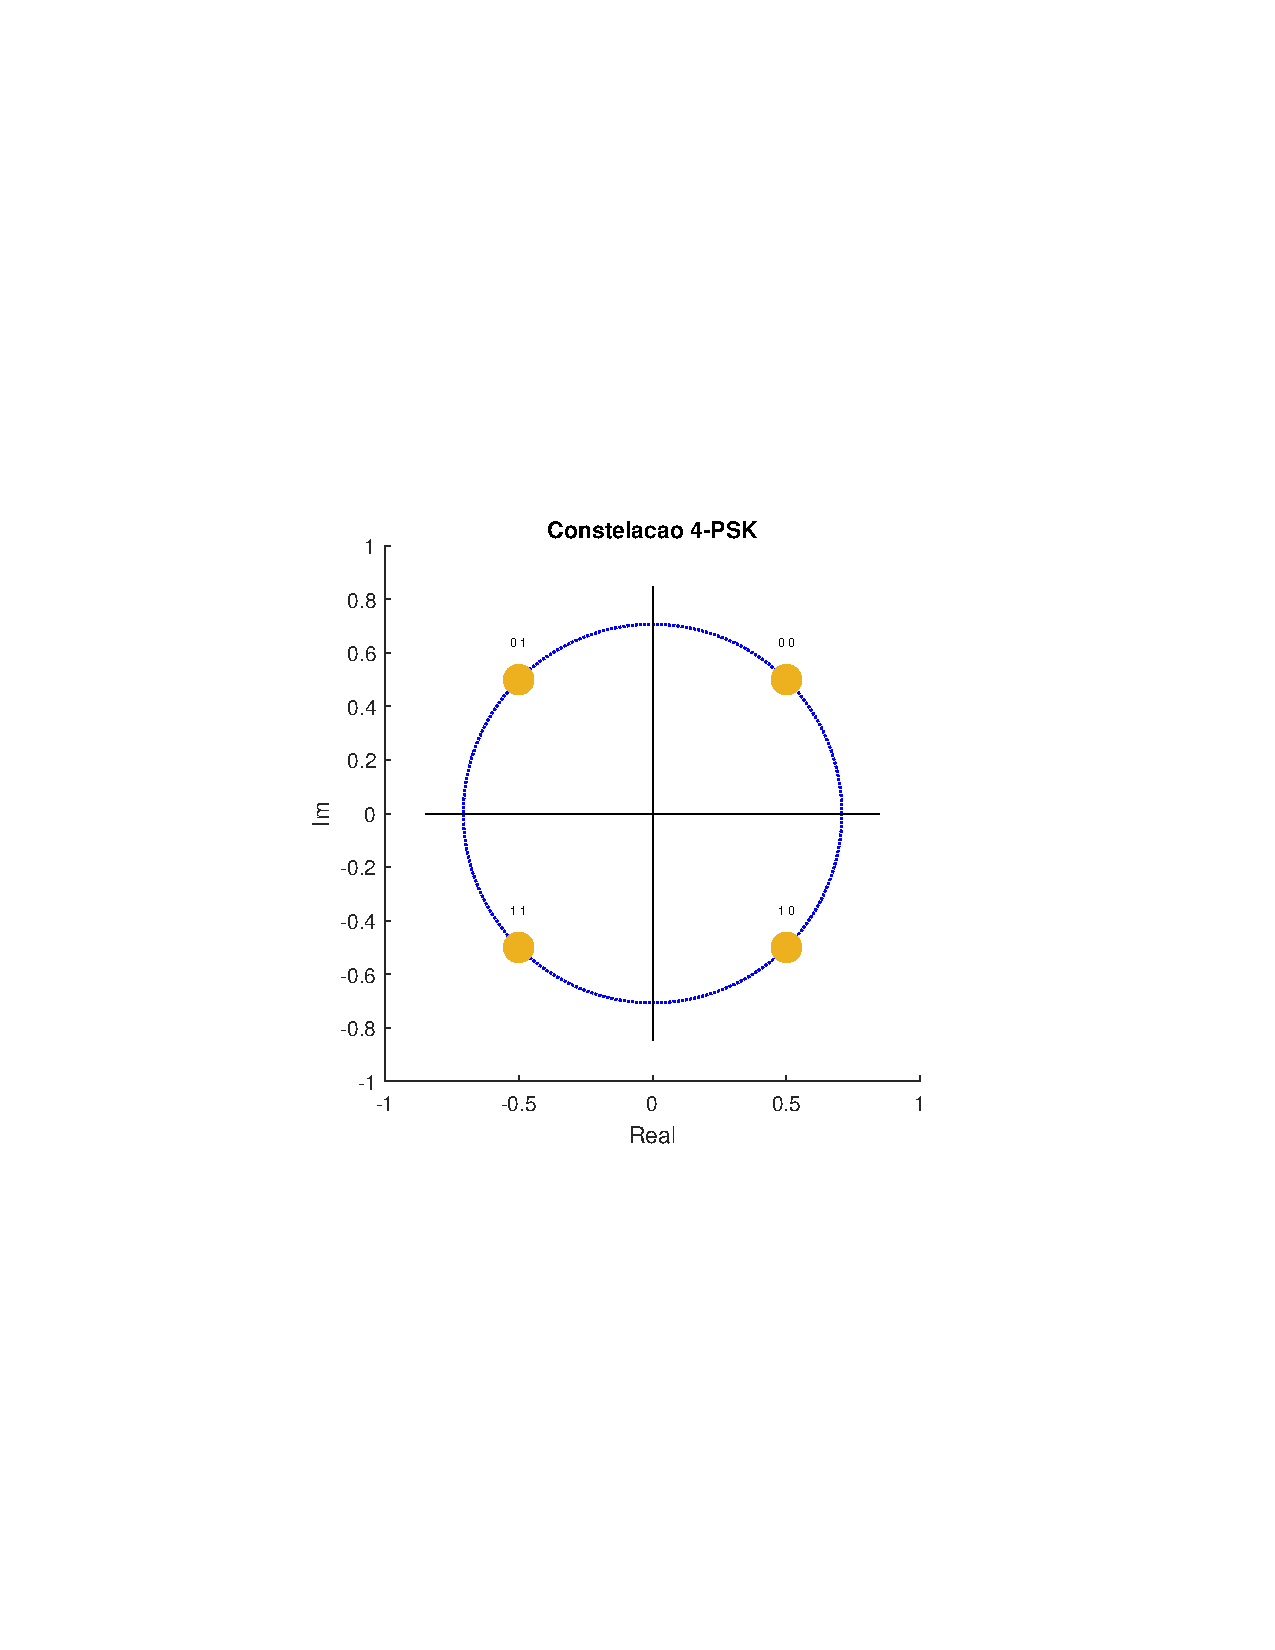
\includegraphics[width=1.0\textwidth,clip=true,trim={1.5cm 8.5cm 1.8cm 8.3cm}]{C:/Users/lukin/Documents/GitHub/Courses-HWs/Sistemas de Comunicacoes Digitais/matlab/problema4/parte1/fig/4_PSK_plot.pdf}
    \caption{Constelação $4$-PSK com codificação de Gray.}
    \label{fig:4_PSK_plot}
\end{figure}

\begin{figure}[!ht]
    \centering
    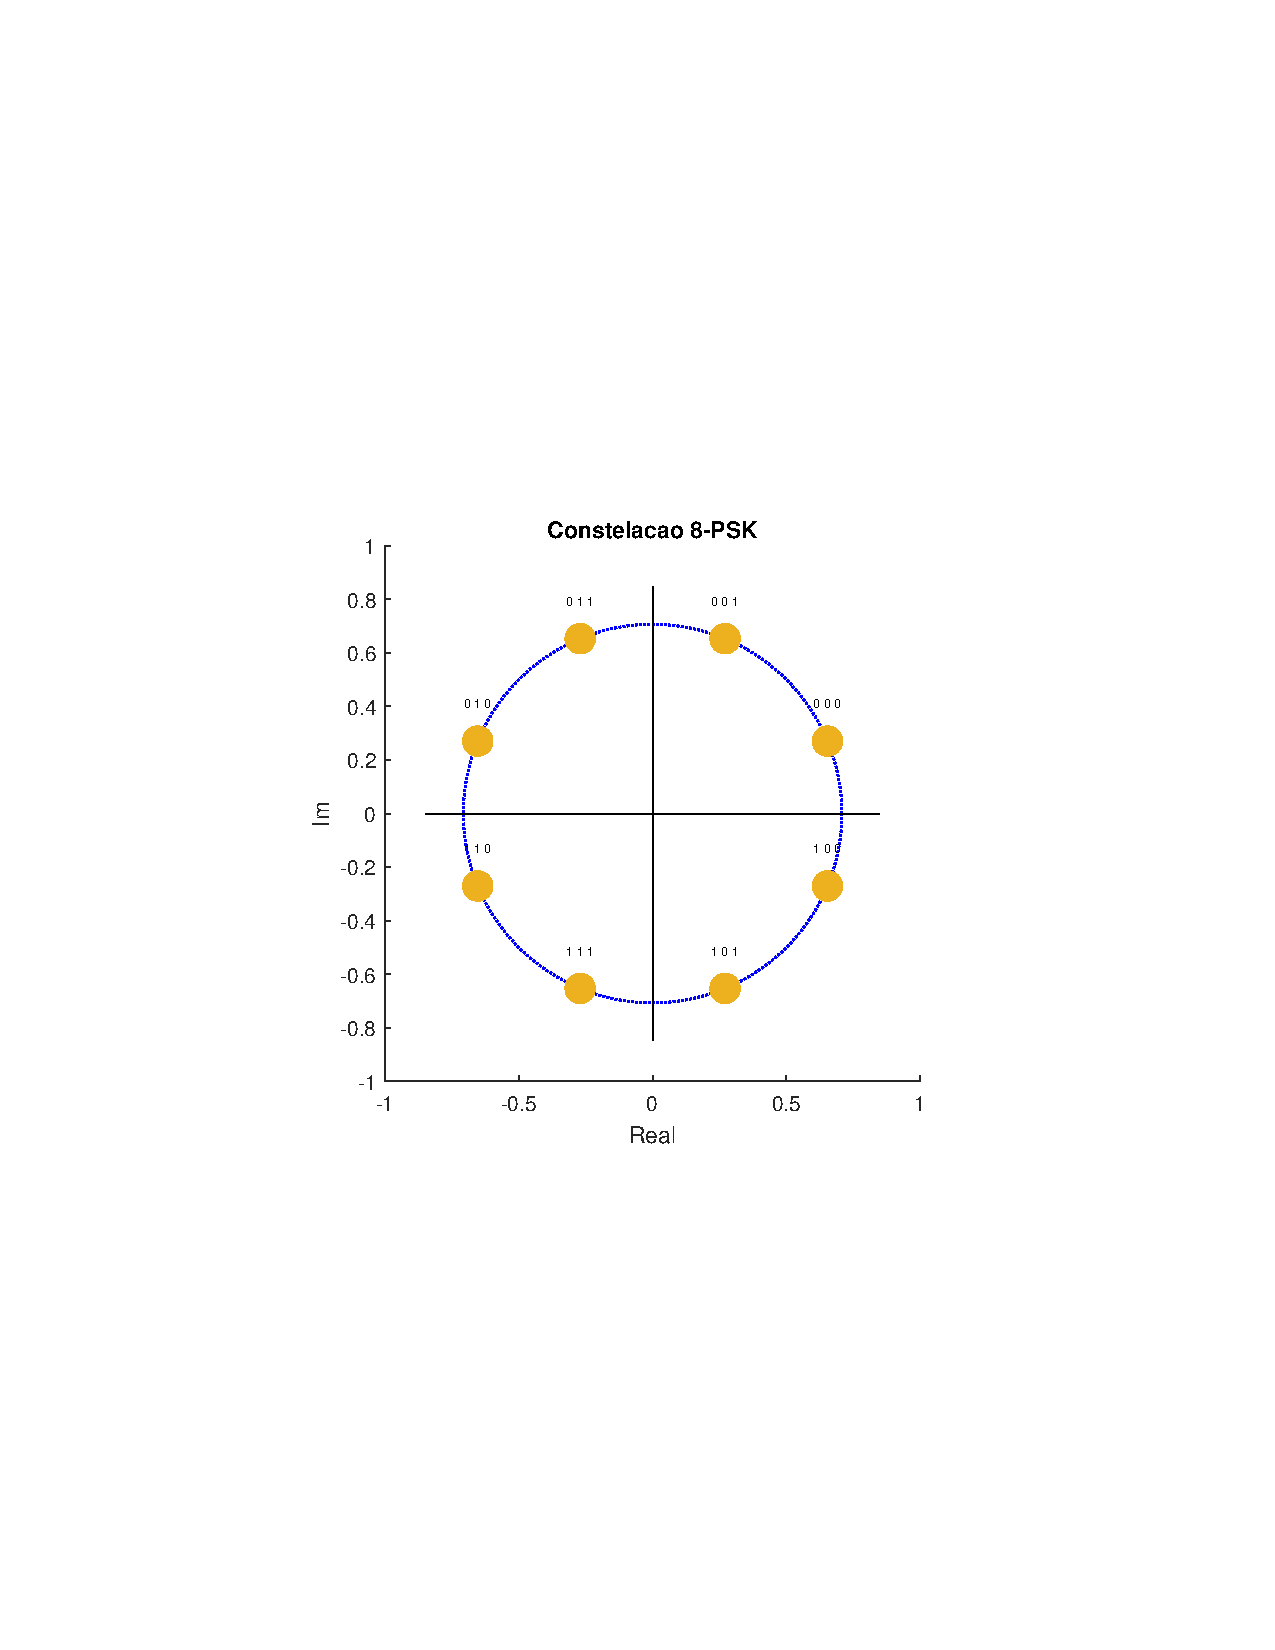
\includegraphics[width=1.0\textwidth,clip=true,trim={1.5cm 8.5cm 1.8cm 8.3cm}]{C:/Users/lukin/Documents/GitHub/Courses-HWs/Sistemas de Comunicacoes Digitais/matlab/problema4/parte1/fig/8_PSK_plot.pdf}
    \caption{Constelação $8$-PSK com codificação de Gray.}
    \label{fig:8_PSK_plot}
\end{figure}



\begin{figure}[!ht]
    \centering
    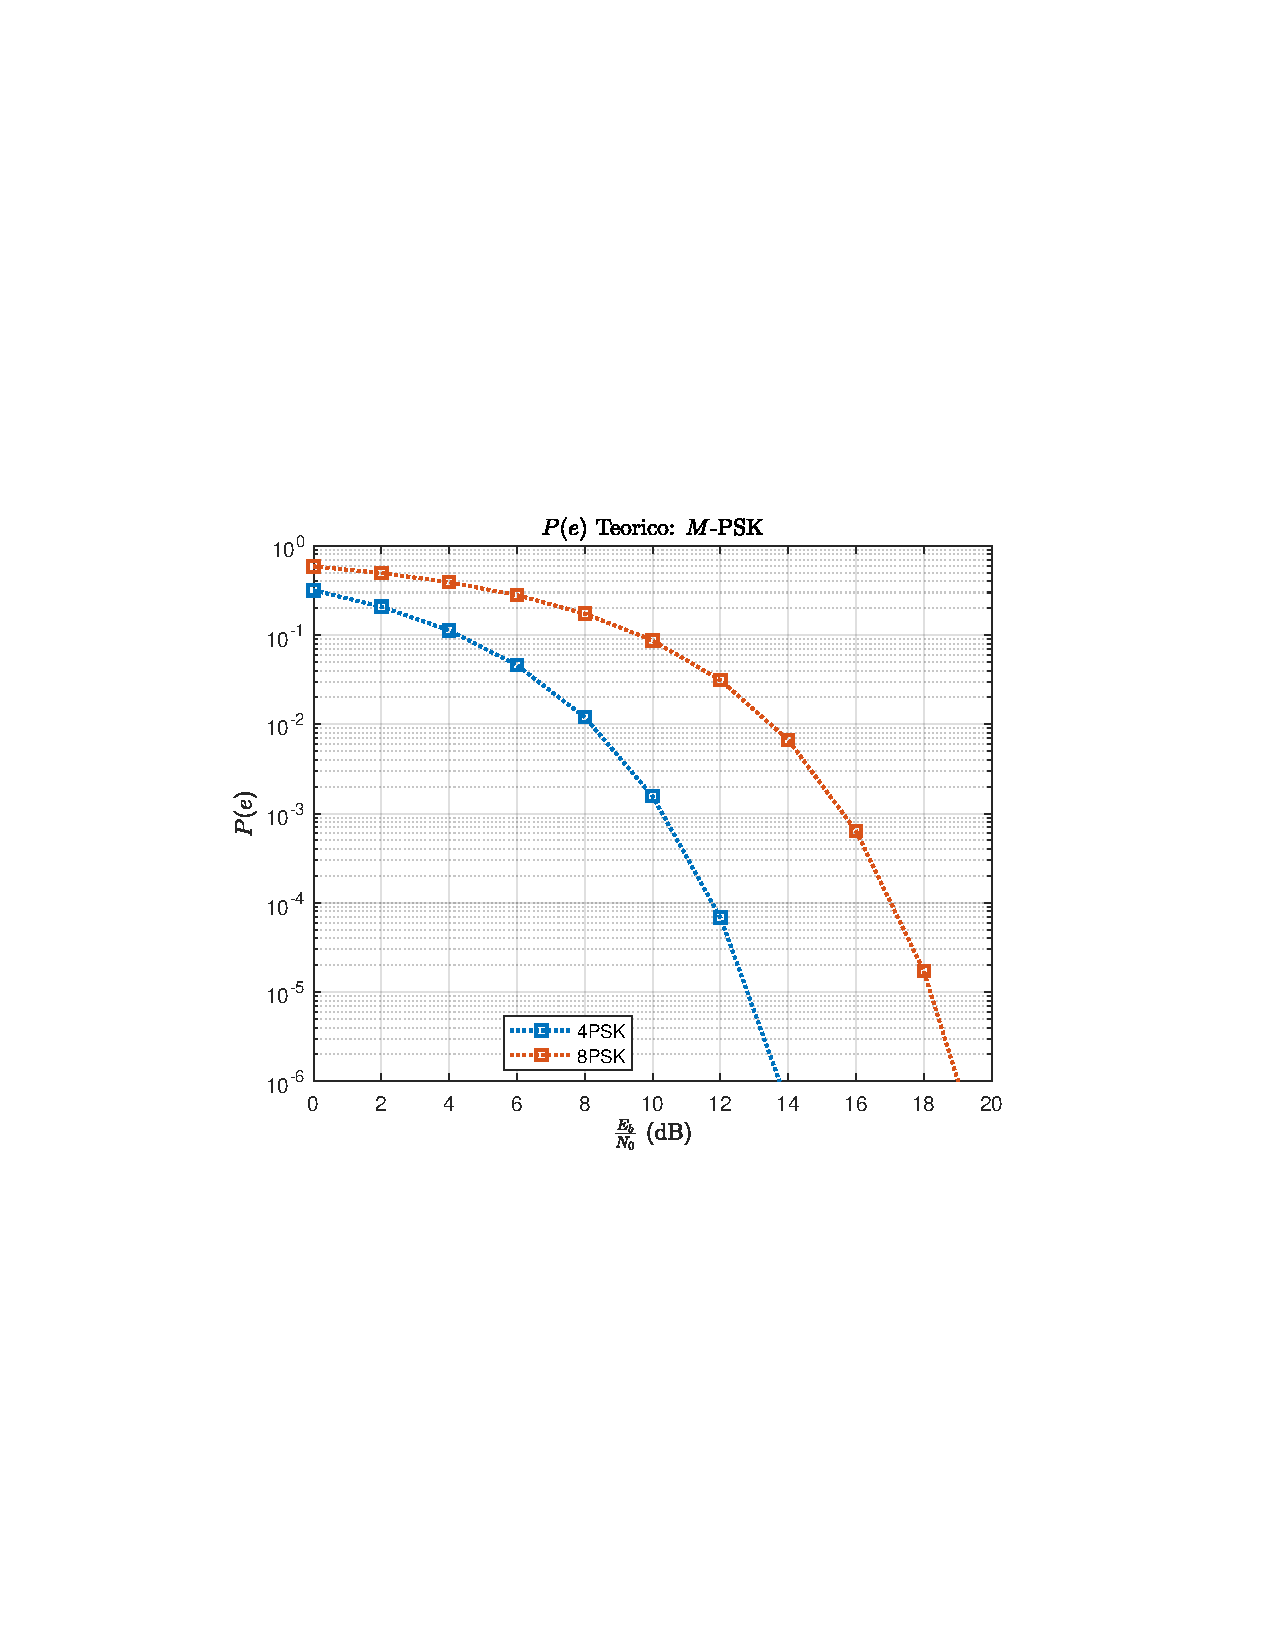
\includegraphics[width=1.0\textwidth,clip=true,trim={1.5cm 8.5cm 1.8cm 8.3cm}]{C:/Users/lukin/Documents/GitHub/Courses-HWs/Sistemas de Comunicacoes Digitais/matlab/problema4/parte2/fig/Erro_Teorico_MPSK.pdf}
    \caption{Probabilidade de erro $(P(e))$ teórico $M$-PSK.}
    \label{fig:Erro_Teorico_MPSK}
\end{figure}


\begin{figure}[!ht]
    \centering
    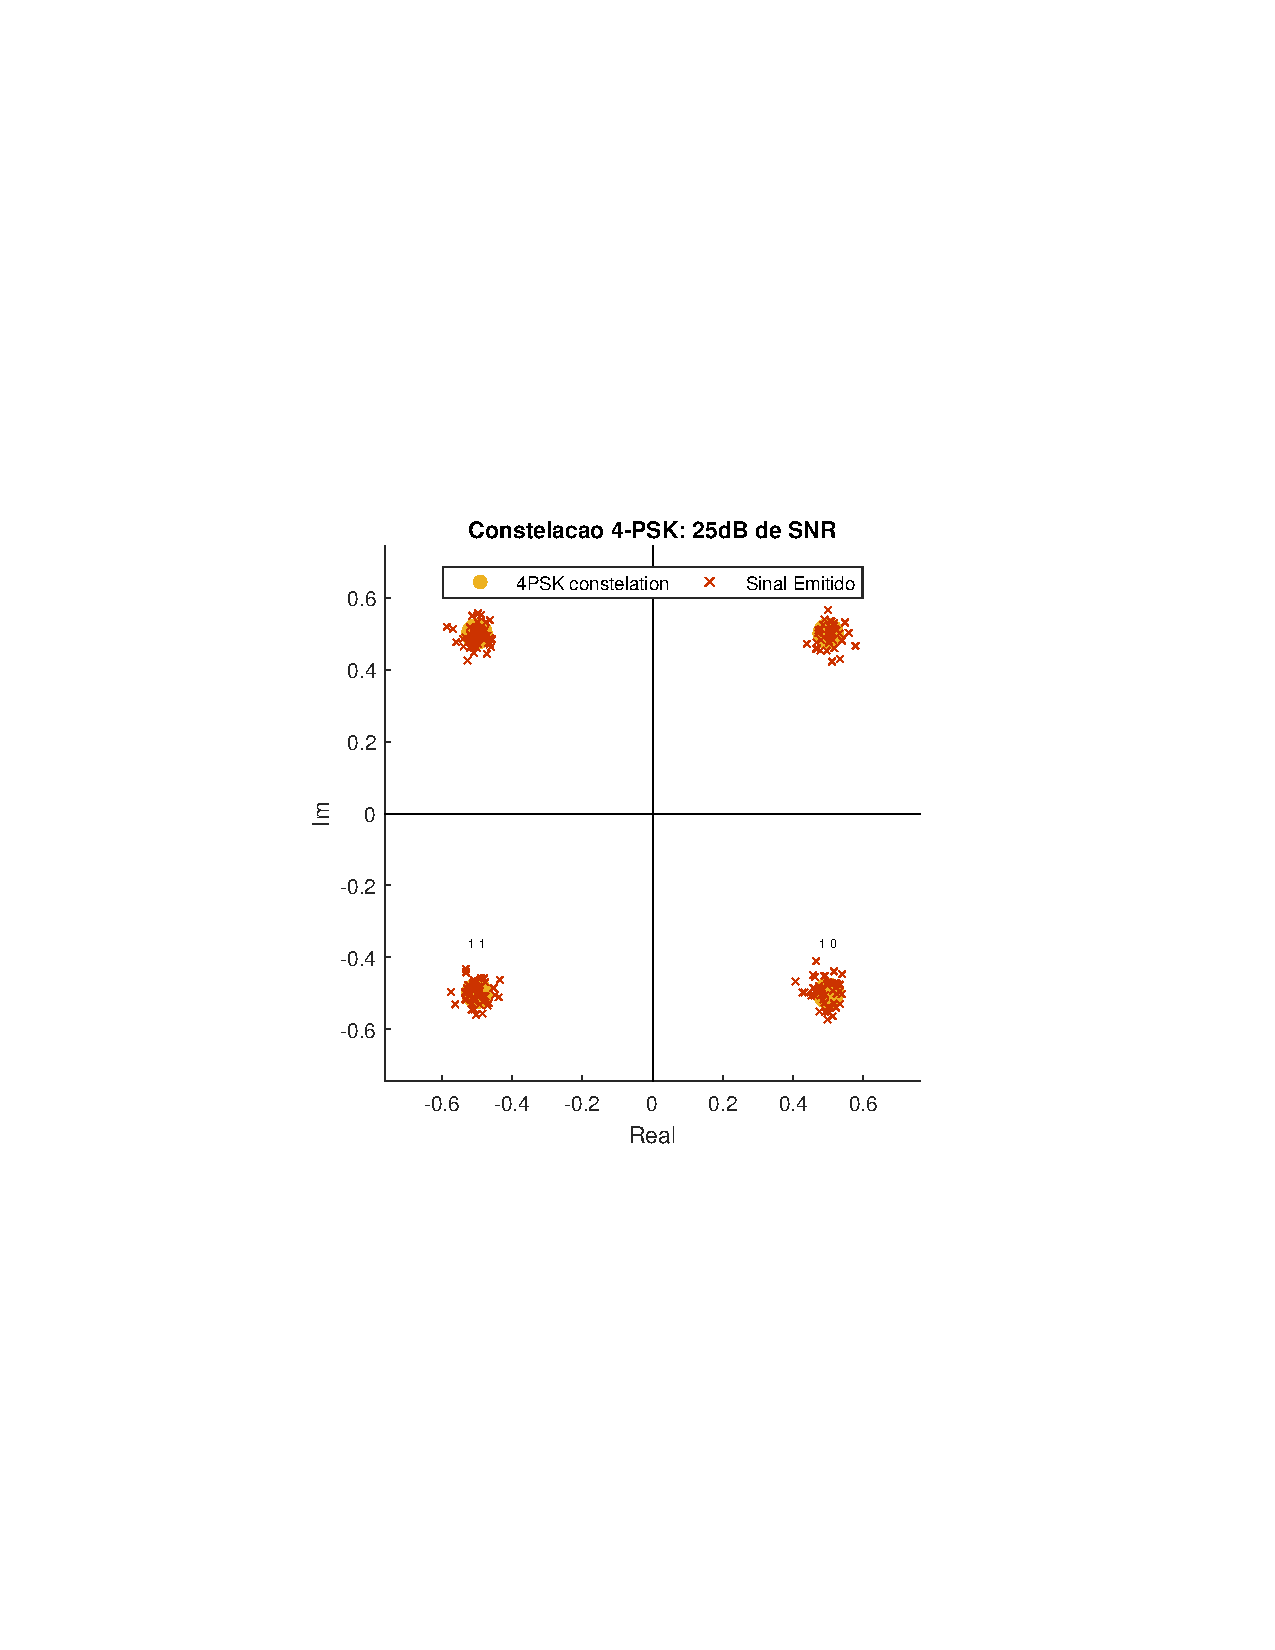
\includegraphics[width=1.0\textwidth,clip=true,trim={1.5cm 8.5cm 1.8cm 8.3cm}]{C:/Users/lukin/Documents/GitHub/Courses-HWs/Sistemas de Comunicacoes Digitais/matlab/problema4/parte3/fig/4PSK_25dB.pdf}
    \caption{Probabilidade de erro $(P(e))$ teórico $M$-PSK.}
    \label{fig:4PSK_25dB}
\end{figure}

\begin{figure}[!ht]
    \centering
    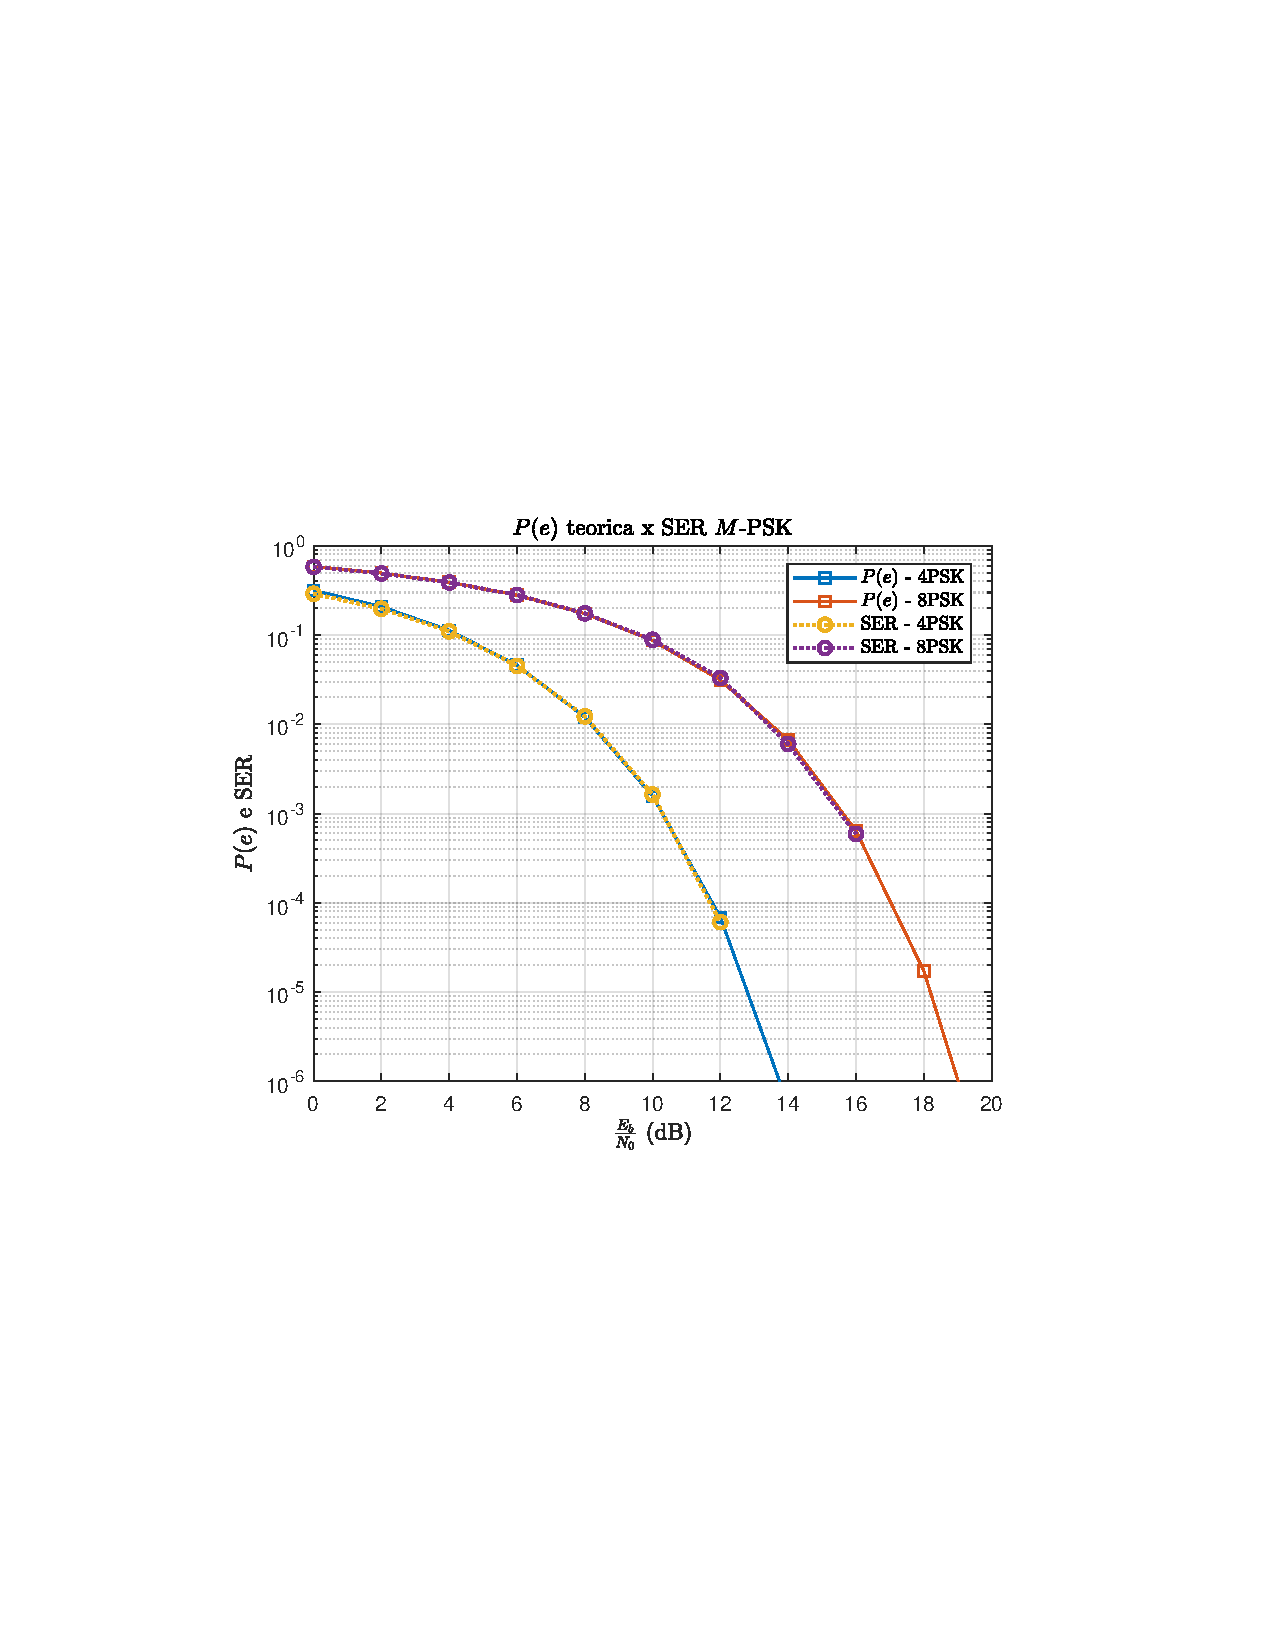
\includegraphics[width=1.0\textwidth,clip=true,trim={1.5cm 8.5cm 1.8cm 8.3cm}]{C:/Users/lukin/Documents/GitHub/Courses-HWs/Sistemas de Comunicacoes Digitais/matlab/problema4/parte3/fig/Erro_teoricaxAWGN_MPSK.pdf}
    \caption{Probabilidade teórica de erro vs. simulação de transmissão $M$-PSK em canal RAGB.}
    \label{fig:Erro_teoricaxAWGN_MPSK}
\end{figure}


\clearpage
\section{Problema 5 - Comparativo \texorpdfstring{$M$}{M}-QAM x \texorpdfstring{$M$}{M}-PSK}

\begin{figure}[!ht]
    \centering
    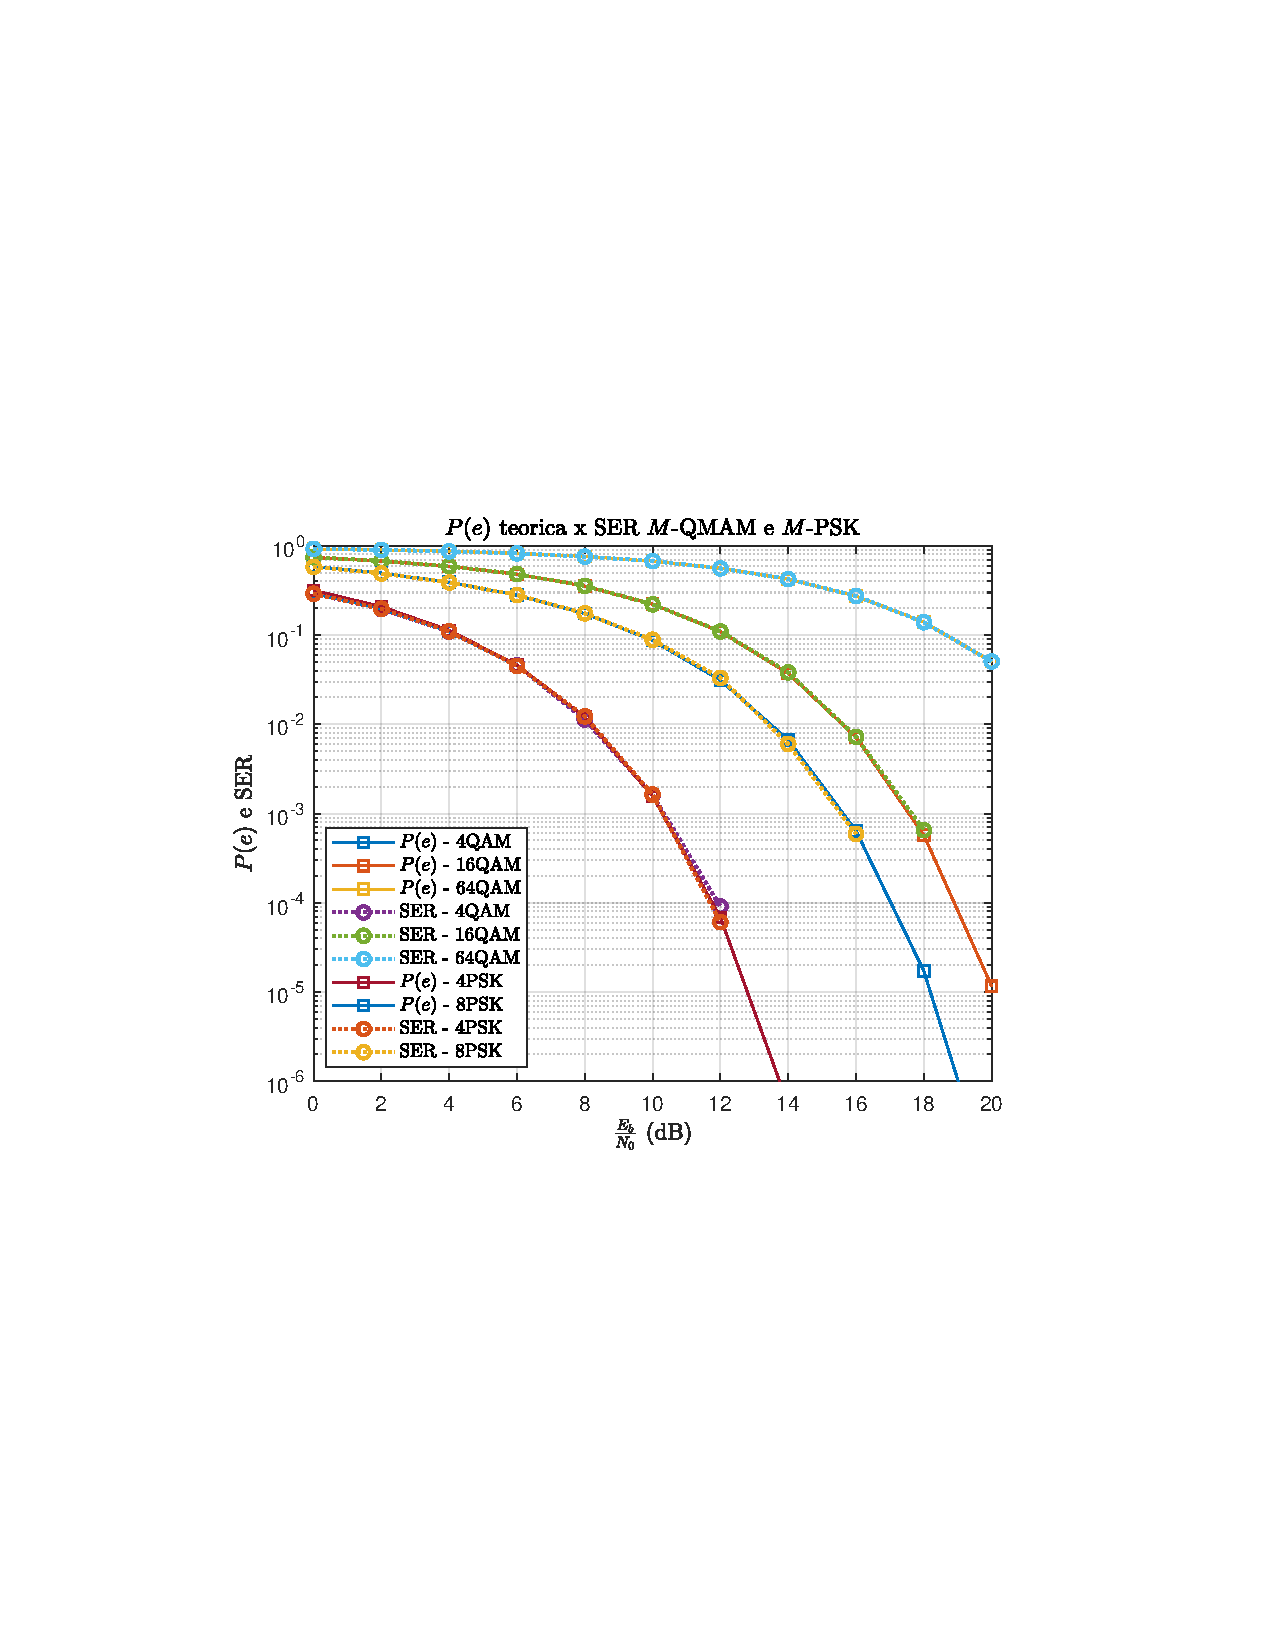
\includegraphics[width=1.0\textwidth,clip=true,trim={1.5cm 8.5cm 1.8cm 8.3cm}]{C:/Users/lukin/Documents/GitHub/Courses-HWs/Sistemas de Comunicacoes Digitais/matlab/problema5/fig/Erro_teoricaxAWGN_Geral.pdf}
    \caption{Probabilidade teórica de erro vs. simulação de transmissão $M$-PSK em canal RAGB.}
    \label{fig:Erro_teoricaxAWGN_Geral}
\end{figure}

\begin{figure}[!ht]
    \centering
    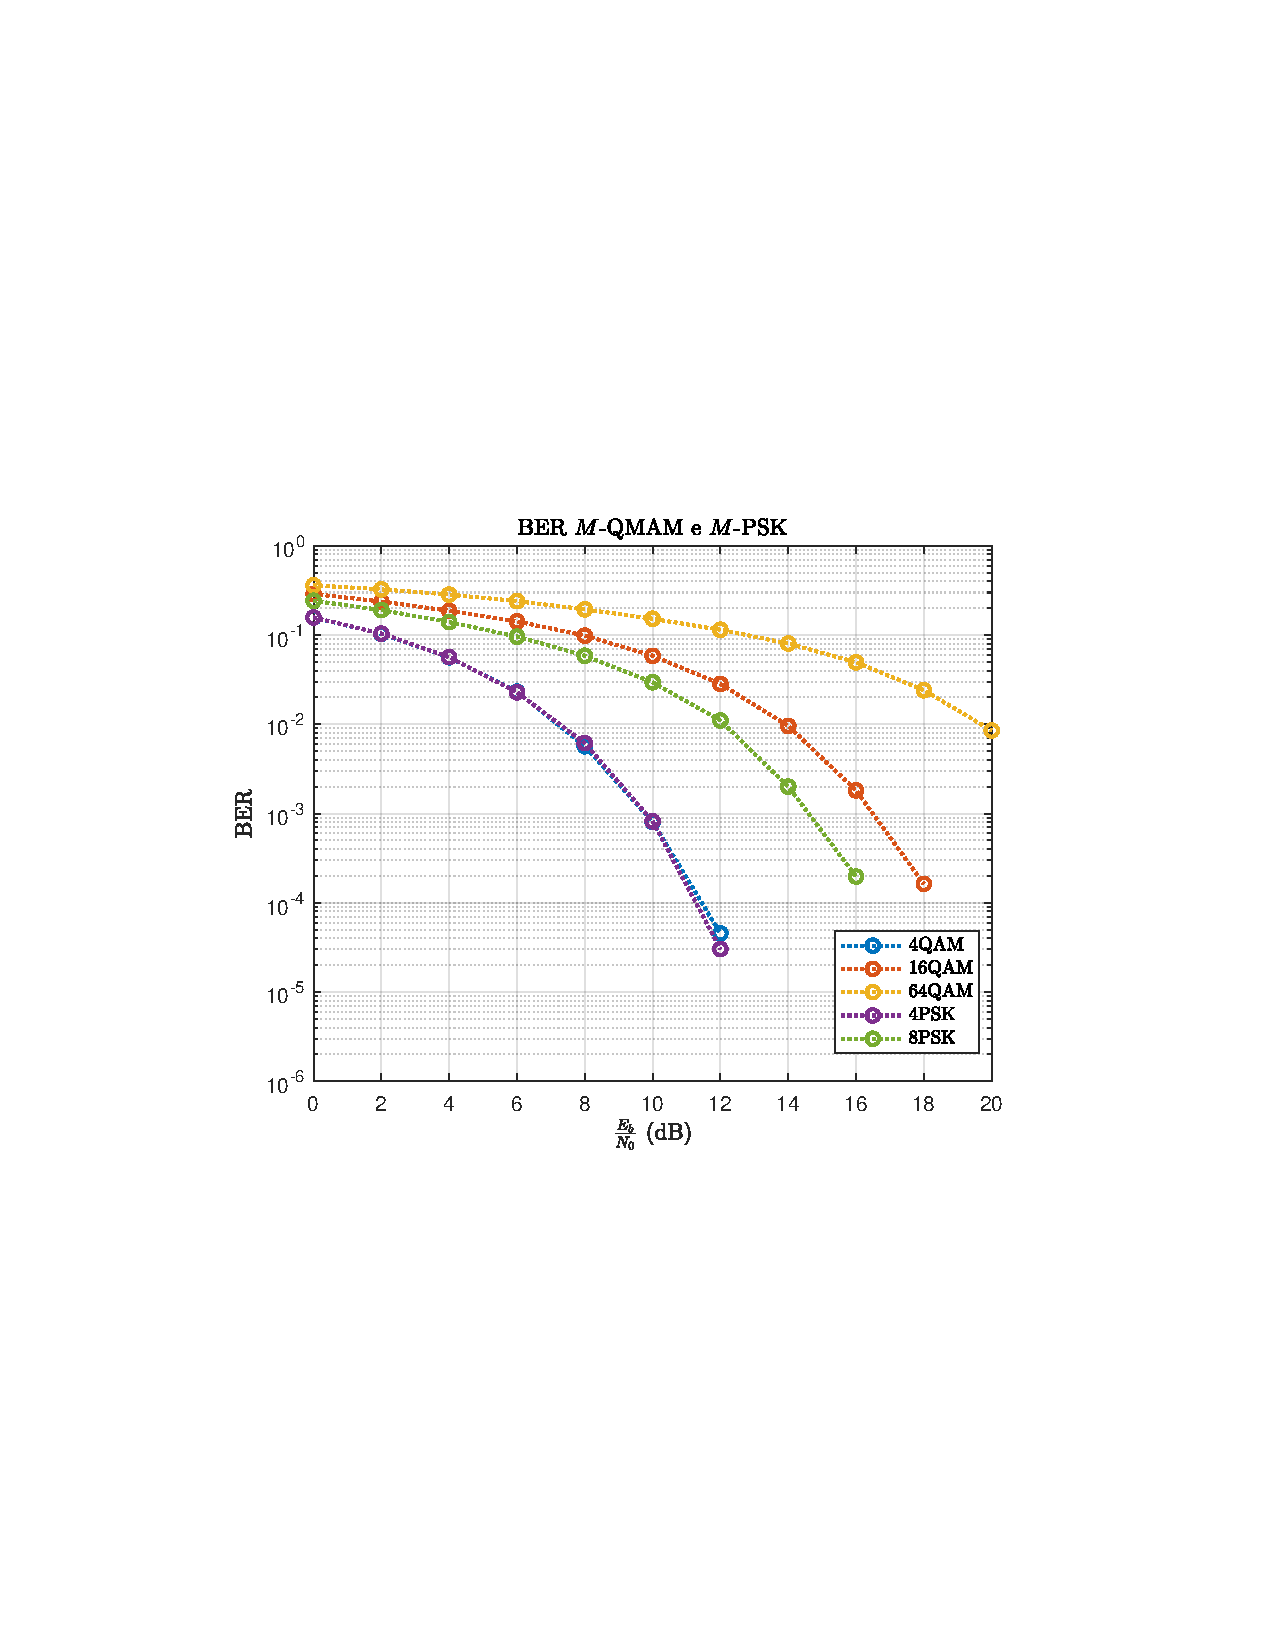
\includegraphics[width=1.0\textwidth,clip=true,trim={1.5cm 8.5cm 1.8cm 8.3cm}]{C:/Users/lukin/Documents/GitHub/Courses-HWs/Sistemas de Comunicacoes Digitais/matlab/problema5/fig/BER_teoricaxAWGN_Geral.pdf}
    \caption{Probabilidade teórica de erro vs. simulação de transmissão $M$-PSK em canal RAGB.}
    \label{fig:BER_teoricaxAWGN_Geral}
\end{figure}


\clearpage

\section{Conclusão e Resultados}
% A título de comparação, a tabela desenvolvida em~\cite{Cecilio} serve para correr os resultados obtidos na simulação. É possível observar que os valores de relação sinal ruído são bem próximos dos estipulados na literatura.

O para o caso do QAM é possível observar que aumentar o número de símbolos ganhamos em b transmitidos por símbolos, porém a energia média da constelação cresce porporcional mente saindo de 1, no caso de m = 4 e chegando a 21 no caso de m = 64. Além disso a exigência de um sistema de transmissão com mais robustez a ruído, pois é aumentando a quantidade de símbolos a influência do ruído aumenta de forma a a deteriorar totalmente a informação enviada

Podemos observar que ao aumentarmos a quantidade de símbolos na constelação, é necessário mais energia para tal constelação, em ambos os casos, QAM E PSK. Além disso, uma SNR baixa acarreta bastante perda de informação, chegando ao ponto de errar a taxa de 0.5 dos símbolos enviados no caso 64-QAM para 0dB. Esta taxa só é menor que 0.01 para $\dfrac{Eb}{N_o} \geq $ 20dB.

Interessante notar também a diferença entre a taxa de erro de bit e a taxa de símbolo, pois a utilizar a codificação de Gray o símbolos decidido apresenta apenas um bit de diferença símbolos vizinhos, garantindo o quê mesmo ao selecionar um símbolo equivocado a mensagem será afetada de apenas um bit.


\clearpage

% Bibliografia
% LateX vai gerar as ``Referências'' automaticamente
% usando a função \cite{nome} do pacote BibTeX é possível
% "puxar todas as informações do arquivo 'refs.bib'
% O nome do arquivo é o primeiro parâmetro de cada referência
% Um exemplo esta é utilizado na primeira seção
% \AtNextBibliography{\small}             % To set a smaller font size for bibliography
\printbibliography[heading=bibintoc]    % Print the references

\end{document}